\RequirePackage[ngerman=ngerman-x-latest]{hyphsubst}
\documentclass[english,ngerman]{tudscrreprt}
\usepackage{babel}
\usepackage{selinput}
\SelectInputMappings{adieresis={ä},germandbls={ß}}
\usepackage[T1]{fontenc}
\usepackage{fixltx2e}
\usepackage{scrhack}
\usepackage{tudscrsupervisor}
\usepackage{xcolor}
\usepackage{gensymb}

%%%
% Glossar
%
\AfterPackage*{hyperref}{%
	\usepackage[%
		automake,% Alphabetische Sortierung, da xindy aktiv, kein makeindex benötigt
		% mit Tex Live einfach verwendbar
		xindy={language=german-din}, % Alphabetische Sortierung nach UTF-8 und Duden oder DIN.
		acronym,% Abkürzungen
		symbols,% Formelzeichen
		%nomain,% kein Glossar
		translate=babel,% Überschriften der Glossare in der Dokumentsprache gesetzt
		nogroupskip,% automatischer Abstand zwischen den Einträgen zur Gruppierung innerhalb eines Glossars entfernen
		toc,% fügt die Verzeichnisse dem Inhaltsverzeichnis hinzu
		section=chapter,% bestimmt die Gliederungsebene der Überschrift
	]{glossaries}
	\makeglossaries
	
\newglossarystyle{acrotabu}{%
	\renewenvironment{theglossary}{%
		\begin{tabu}spread 0pt{@{}lX<{\strut}l@{}}%
	}{%
		\end{tabu}\par\bigskip%
	}%
	\renewcommand*{\glossaryheader}{}%
	\renewcommand*{\glsgroupheading}[1]{}%
	\renewcommand*{\glsgroupskip}{}%
	\renewcommand*{\glossentry}[2]{%
		\glsentryitem{##1}% Entry number if required
		\glstarget{##1}{\sffamily\bfseries\glossentryname{##1}} &
		\glsentrydesc{##1} &
		##2\tabularnewline
	}
}

\newcommand*{\newsymbol}[5][]{%
	\newglossaryentry{#2}{%
		type=symbols,%
		description={},%
		name={#3},%
		symbol={\ensuremath{#4}},%
		user1={\ensuremath{\mathrm{#5}}},%
		sort={#2},%
		#1%
	}%
}

\defglsentryfmt[symbols]{%
	\ifmmode%
	\glssymbol{\glslabel}%
	\else%
	\glsgenentryfmt~\glsentrysymbol{\glslabel}%
	\fi%
}
\newglossarystyle{symblongtabu}{%
	\renewenvironment{theglossary}{%
		\begin{longtabu}spread 0pt[l]{ccX<{\strut}l}%
		}{%
		\end{longtabu}%
	}%
	\renewcommand*{\glossaryheader}{%
		\toprule
		\bfseries Symbol & \bfseries Einheit &
		\bfseries Name & \bfseries Seite(n)
		\tabularnewline\midrule\endhead%
		\bottomrule\endfoot%
	}%
	\renewcommand*{\glsgroupheading}[1]{}%
	\renewcommand*{\glsgroupskip}{}%
	\renewcommand*{\glossentry}[2]{%
		\glsentryitem{##1}% Entry number if required
		\glstarget{##1}{\glossentrysymbol{##1}} &
		\glsentryuseri{##1} &
		\glossentryname{##1} &
		##2\tabularnewline%
	}%
}
}% Ende von AfterPackage*

%%%
% Zitate
%
\usepackage{csquotes}
\usepackage[backend=biber,style=alphabetic]{biblatex}
\addbibresource{bib/MMandCountourTrees.bib}
\addbibresource{bib/Polyeder.bib}

%%%
% Caption
%
\usepackage{caption}
\captionsetup{font=sf,labelfont=bf,labelsep=space}
\usepackage{floatrow}
\floatsetup{font=sf}
\floatsetup[table]{style=plaintop}
\captionsetup{singlelinecheck=off,format=hang,justification=raggedright}
\DeclareCaptionSubType[alph]{figure}
\DeclareCaptionSubType[alph]{table}
\captionsetup[subfloat]{labelformat=brace,list=off}

%%%
% Tabellen
%
\usepackage{booktabs} % Linien für Tabellen.
\usepackage{array} % Definitionen für Spalten.
\usepackage{tabularx} % Tabellen mit gleicher Spaltenbreite.
\usepackage{tabulary}
\usepackage{tabu}


%%%
% Index
%
\usepackage{imakeidx}
\indexsetup{%
	level=\chapter*,
	noclearpage, firstpagestyle=headings, headers={\indexname}{\indexname},
	othercode={\renewcommand*\subitem{\@idxitem\hspace*{15\p@}}}
}\makeindex

%%%
% Bilder
%
\usepackage{graphicx}
\graphicspath{ {./media/} }

%%%
% Quellcode
%
\usepackage{listings}
% UTF8
\lstset{%
	inputencoding = utf8,
	extendedchars = true, % lets you use non-ASCII characters; for 8-bits encodings only, does not work with UTF-8
	literate=%
	{ä}{{\"a}}1 {ö}{{\"o}}1 {ü}{{\"u}}1
	{Ä}{{\"A}}1 {Ö}{{\"O}}1 {Ü}{{\"U}}1
	{~}{{\textasciitilde}}1 {ß}{{\ss}}1
}
\definecolor{dkgreen}{rgb}{0,0.6,0}
\definecolor{mygray}{rgb}{0.5,0.5,0.5}
\definecolor{mymauve}{rgb}{0.58,0,0.82}
\lstset{ %
	backgroundcolor=\color{white},   % choose the background color; you must add \usepackage{color} or \usepackage{xcolor}
	basicstyle=\footnotesize,        % the size of the fonts that are used for the code
	breakatwhitespace=false,         % sets if automatic breaks should only happen at whitespace
	breaklines=true,                 % sets automatic line breaking
	captionpos=b,                    % sets the caption-position to bottom
	commentstyle=\color{dkgreen},    % comment style
	deletekeywords={...},            % if you want to delete keywords from the given language
	escapeinside={\%*}{*)},          % if you want to add LaTeX within your code
	frame=single,                    % adds a frame around the code
	keepspaces=true,                 % keeps spaces in text, useful for keeping indentation of code (possibly needs columns=flexible)
	keywordstyle=\color{blue},       % keyword style
	language=Octave,                 % the language of the code
	morekeywords={*,...},            % if you want to add more keywords to the set
	numbers=left,                    % where to put the line-numbers; possible values are (none, left, right)
	numbersep=5pt,                   % how far the line-numbers are from the code
	numberstyle=\tiny\color{mygray}, % the style that is used for the line-numbers
	rulecolor=\color{black},         % if not set, the frame-color may be changed on line-breaks within not-black text (e.g. comments (green here))
	showspaces=false,                % show spaces everywhere adding particular underscores; it overrides 'showstringspaces'
	showstringspaces=false,          % underline spaces within strings only
	showtabs=false,                  % show tabs within strings adding particular underscores
	stepnumber=2,                    % the step between two line-numbers. If it's 1, each line will be numbered
	stringstyle=\color{mymauve},     % string literal style
	tabsize=2,                       % sets default tabsize to 2 spaces
	title=\lstname                   % show the filename of files included with \lstinputlisting; also try caption instead of title
}

%%%
% Links
%
\usepackage{hyperref} % Möglichst am Ende stehen, da es viele Befehle neu definiert.
\hypersetup{
	colorlinks   = true, %Colours links instead of ugly boxes
	urlcolor     = HKS41!70, %Colour for external hyperlinks
	linkcolor    = HKS44!70, %Colour of internal links
	citecolor    = HKS33!80 %Colour of citations
}

\usepackage{quoting}

\usepackage[babel]{microtype}

\usepackage{xfrac}

%%%
% Aufzählungen
%
\usepackage{enumitem}
\setlist[itemize]{noitemsep}
\setlist[description]{noitemsep}

\usepackage{isodate}

\usepackage{ellipsis}
\let\ellipsispunctuation\relax

\usepackage{amssymb} % Muss nach hyperref kommen, sonst Fehler "\newsymbol already defined". Alternative: http://tex.stackexchange.com/questions/73684/are-there-any-situtations-where-it-is-better-to-load-a-package-after-other-code

\usepackage{tikz}
\usetikzlibrary{arrows,positioning,scopes,trees}
%%%
% Index
%
\newcommand{\CFD}{\gls{cfd}\index{CFD-Algorithmus}}
\newcommand{\SECC}{\gls{secc}\index{SECC-Algorithmus}}

%Allgemein
\newcommand{\tool}[1]{\textit{#1}\index{#1}} %und libs. Wg vieler Abkürzungen evtl ins Glossar! (z.B. ANN, OpenMP, PPL)
\newcommand{\tools}[2]{\textit{#1}\index{#2}}
\newcommand{\propername}[1]{\textit{#1}\index{#1}} % Allgemein.
\newcommand{\propernames}[2]{\textit{#1}\index{#2}} % Allgemein.
\newcommand{\SEPlugin}[1]{\textit{#1}\index{#1}} % Programmaufbau, evtl in Glossar umwandeln!
\newcommand{\SEPlugins}[2]{\textit{#1}\index{#2}} % Programmaufbau.

%Visualisierung
\newcommand{\visattr}[1]{\textit{#1}\index{#1}}
\newcommand{\visattrs}[2]{\textit{#1}\index{#2}}
\newcommand{\vis}[1]{\textit{#1}\index{#1}} %Visuelles
\newcommand{\viss}[2]{\textit{#1}\index{#2}} %Visuelles
\newcommand{\dataparam}[1]{\textit{#1}\index{#1}}
\newcommand{\dataparams}[2]{\textit{#1}\index{#2}}

% Berechnung
\newcommand{\contour}[1]{\textit{#1}\index{#1}}
\newcommand{\contours}[2]{\textit{#1}\index{#2}}
\newcommand{\SECterm}[1]{\textit{#1}\index{#1}}
\newcommand{\SECterms}[2]{\textit{#1}\index{#2}}
\newcommand{\CFDterm}[1]{\textit{#1}\index{#1}}
\newcommand{\CFDterms}[2]{\textit{#1}\index{#2}}

%%%
% Auszeichnungen
%
\newcommand{\wichtig}[1]{\textit{#1}}
\newcommand{\mrkg}[1]{\textcolor{orange}{#1}} % Markierung, etwa in Gleichungen
\newcommand{\mrkgb}[1]{\textcolor{magenta}{#1}} % Markierung, etwa in Gleichungen
\newcommand{\libNoIndex}[1]{\textit{#1}}

%%%
% Tabelle
%
\newcolumntype{F}{>{\hspace{0pt}}X}
\newcolumntype{L}{>{\raggedright}F}
\newcolumntype{C}{>{\centering}F}
\newcolumntype{D}{>{\centering}F}
\newcolumntype{R}{>{\raggedleft}F}

%%%
% Symbole
%
\newcommand{\kreuz}{ $\times$ }
\newcommand{\esfolgt}{ $\to$ }
\newcommand{\eqtxt}[1]{\stackrel{\text{#1}}{=}} %Gleichheitszeichen mit Text drüber
\newcommand{\intxt}[1]{\stackrel{\text{#1}}{\in}} %Element von mit Text drüber
\newcommand{\abs}[1]{\lvert#1\rvert}
\newcommand{\norm}[1]{\lVert#1\rVert}
\newcommand{\qed}{$_\square$} %Was zu beweisen war; quod erat demonstrandum

%%%
% TikZ
%
\tikzset {
	value/.style={rectangle, draw},
	vocab/.style={rectangle, draw, rounded corners=.8ex},
	verticalChild/.style={grow=down, xshift=.5em, anchor=west, font = \small,
					edge from parent path={(\tikzparentnode.south) |- (\tikzchildnode.west)}},
	first/.style={level distance=6ex},
	second/.style={level distance=12ex},
	third/.style={level distance=18ex},
	fourth/.style={level distance=24ex},
	level 1/.style={sibling distance=3cm}
}
\newglossaryentry{platonischer Körper}{
	name = {platonischer Körper},
	description = {fünf},
	plural = {platonische Körper},
	sort = {Körper}
}

\newglossaryentry{3dRaum} {
	name = {\ensuremath{\mathbb{R}^3}},
	description = {Dreidimensionaler Raum},
	sort = {R}
}

\newacronym[
	longplural={Relationale Datenbankmanagementsysteme}
	description={Relationales Datenbankmanagementsystem}
]{rdbms}{RDBMS}{Relationalen Datenbankmanagementsystems}

\newacronym[
	longplural={Hue-Saturation-Brightness}
	description={Ein Farbschema mit drei Dimensionen für Farbwert (0°-360°), Sättigung und Helligkeit.}
]{hsb}{HSB}{Hue-Saturation-Brightness}



\newacronym[
	longplural={Pixel}
	description={Eine Einheit.}
]{px}{px}{Pixel}



\newacronym[
longplural={MegaMol Structure Events}
description={Das Dateiformat für die Structure Events.}
]{mmse}{MMSE}{MegaMol Structure Event}

\newacronym[
longplural={Structure Events Cluster Compare}
description={Vergleich von Clustern über zwei Frames.}
]{secc}{SECC}{Structure Events Cluster Compare}

\newacronym[
longplural={Structure Events Data Call}
description={Der MegaMol Call, der zum Übertragen von Structure Events Daten genutzt wird.}
]{sedc}{SEDC}{Structure Events Data Call}

%\usepackage{tudscrman}

\begin{document}

\faculty{Fakultät für Informatik}
%\department{Institut für Systemarchitektur}
\institute{Institut für Systemarchitektur}
\chair{Professur für Datenbanken}

\subject{Arbeitsname Bachelorarbeit}
%\subject{bachelor}
\title{Visualisierung von Clusterereignissen bei der Expansion eines idealen Gases im Vakuum}
\thesis{Bachelor WIP}
%\thesis{bachelor}

\graduation[B.Sc.]{Bachelor of Science}
\author{%
	Richard Hähne
	\matriculationnumber{2873574}
	\dateofbirth{10.2.1982}
	\placeofbirth{Dresden}
	\matriculationyear{2011}
	\course{Medieninformatik}
	%\discipline{Informationsvisualisierung}
}

%\referee{Dr. Grottel}
\supervisor{Sebastian Grottel \and Ludwig Schmutzler}
\professor{Prof. Dr. Stefan Gumhold}
\date{2945-12-31}
%\defensedate{2945-12-31}

%\frontmatter %Vorspann: Römische Seitennummerierung

%\makecover
\maketitle

\TUDoption{abstract}{section,multiple}
\begin{abstract}
	Das vorliegende Dokument befindet sich im grundlegenden Aufbau. Fokus ist eine schnelle Erfassbarkeit bestimmter Inhalte, so dass eher Aufzählungen und Tabellen zu finden sind, die in der Veröffentlichungsfassung gegen Fließtext eingetauscht werden.
	
	WIP gilt auch für Layout und Farben.
	
	Großgeschriebene Wortgruppen sind Erinnerungen an mich.
\end{abstract}

%\declaration \tableofcontents \listoffigures \listoftables

\printacronyms[style=acrotabu] \printsymbols[style=symblongtabu]

%\mainmatter %Hauptteil: Normale Seitennummerierung


\chapter{Grundlagen}

Reminder an mich: Inhaltsplanung begrenzen! Es wird schon viel zuviel für ne BA, wenn noch Molekularzeugs/Vergleich mit anderen Arbeiten mit reinkommen sollte.

\begin{itemize}
\item Präattentive Wirkung visueller Variablen (für Priorisierungsreihenfolge visueller Attribute in \autoref{sec:attribute} sowie die Nutzung für Agglomerate). Räumliche Verknüpfungen sind oftmals präattentiv, z.B. Bewegung und (Farbe | Form| 3D-Disparität). Die meisten Verknüpfungen sind nicht präattentiv. => Nutzung möglichst weniger Variablen fördert präattentive Informationsaufnahme =>  Mehrfachzuweisung (Farbe und Form für Zeit z.B.) vermeiden, auch wenn sie scheinbar zur Verstärkung beitragen.
\item falls visuelle Relationen vorkommen: Beispiele von Netzwerken
\item falls Zoom eine Rolle spielt: Ansichten, siehe KP InfVis
\end{itemize}

Zwischenpräsi Mitte Mai.
Treffen Mo 13-14.

\section{Contour Tree}

\blockcquote[1]{ComputingContourTrees}{Isolines, often called contours, are the curves consisting of points at a given height that can be seen on any topographic map.}

\blockcquote[2]{ComputingContourTrees}{We refer to the vertices and edges of the contour tree as supernodes and superarcs, respectively.}

level set = Niveaumenge: Menge aller Punkte einer Funktion (eines Skalarfelds), denen der gleiche Wert zugeordnet ist.

Contour/Isolinie -> Join and Split Tree -> Merge -> Contour Tree (2D oder 3D? glaub 3D) \cite[S.~1]{ContourTreeAlgorithm}

Join: von oben nach unten, Split: von unten nach oben \cite{ContourTreeJoinSplit}

\section{Ereigniserkennung}
Partikel hat ID (durch Arrayindex). Partikel in Zeitschritt 1 \& 2 einem Cluster zuordnen und schauen, ob es sich
\begin{itemize}
	\item im selben, (kann Merge sein, wenn andere Partikel hinzu)
	\item einem anderen schon bei Zeitschritt 1 vorhandenen, (Split)
	\item einem neuen (Split/Birth)
\end{itemize}
Cluster befindet. Es können auch auf denselben Clustern mehrere Ereignisse passieren.

\section{Visualisierung}


\section{Gestaltgesetze}\label{sec:gestaltgesetze}
QUELLEN HINZUFÜGEN,  siehe V InfVis, V Gestaltung.

DER EINFACHHEIT HALBER COPYPASTE WIKI, DA NOCH NICHT KLAR, WAS TATSÄCHLICH GEBRAUCHT:
\begin{description}
\item [Gesetz der Prägnanz]
Es werden bevorzugt Gestalten wahrgenommen, die sich von anderen durch ein bestimmtes Merkmal abheben (Prägnanztendenz). Jede Figur wird so wahrgenommen, dass sie in einer möglichst einfachen Struktur resultiert (= „Gute Gestalt“).
\item [Gesetz der Nähe]
Elemente mit geringen Abständen zueinander werden als zusammengehörig wahrgenommen.
\item [Gesetz der Ähnlichkeit]
Einander ähnliche Elemente werden eher als zusammengehörig erlebt als einander unähnliche.
\item [Gesetz der Kontinuität]
Reize, die eine Fortsetzung vorangehender Reize zu sein scheinen, werden als zusammengehörig angesehen.
\item [Gesetz der Geschlossenheit]
Linien, die eine Fläche umschließen, werden unter sonst gleichen Umständen leichter als eine Einheit aufgefasst als diejenigen, die sich nicht zusammenschließen (D. Katz, Gestaltpsychologie, 1969).
\item [Gesetz der gemeinsamen Bewegung]
Zwei oder mehrere sich gleichzeitig in eine Richtung bewegende Elemente werden als eine Einheit oder Gestalt wahrgenommen.
\item [Gesetz der fortgesetzt durchgehenden Linie]
Linien werden immer so gesehen, als folgten sie dem einfachsten Weg. Kreuzen sich zwei Linien, so gehen wir nicht davon aus, dass der Verlauf der Linien an dieser Stelle einen Knick macht, sondern wir sehen zwei gerade durchgehende Linien.
Zusätzlich zu diesen von Wertheimer formulierten Gesetzen fand Stephen Palmer in den 1990er Jahren drei weitere Gestaltgesetze.[1]

\item [Gesetz der gemeinsamen Region]
Elemente in abgegrenzten Gebieten werden als zusammengehörig empfunden.
\item [Gesetz der Gleichzeitigkeit]
Elemente, die sich gleichzeitig verändern, werden als zusammengehörig empfunden.
\item [Gesetz der verbundenen Elemente]
Verbundene Elemente werden als ein Objekt empfunden.
\end{description}

\section{Formgebung}\label{sec:grundlagen:formgebung}
Eine einfache Möglichkeit, unterschiedliche Formen aus einer runden Grundform zu erzeugen, ist ein Zylinder mit nach außen führenden Spitzen wie bei einem Stern, was einem nichtkonvexen Prisma entspricht \cite{UniformPolyhedra}. Wie in \autoref{fig:formen:sterne3d} zu sehen, sind die Sternformen von vorn und hinten gut zu unterscheiden. Von der Seite und von oben fällt die Abgrenzung voneinander jedoch schwerer. Weiterhin haben die Elemente in der Seitenansicht eine andere Erscheinung als in der Frontalansicht, so dass dadurch die Verknüpfung zwischen beiden Ansichten mit zusätzlichem kognitiven Aufwand verbunden ist. Deswegen ist diese Art der Formgebung für eine 3D Ansicht nicht geeignet.

\begin{figure}
	\ffigbox[\FBwidth] {
		\begin{subfloatrow}
			\ffigbox[\FBwidth][]
				{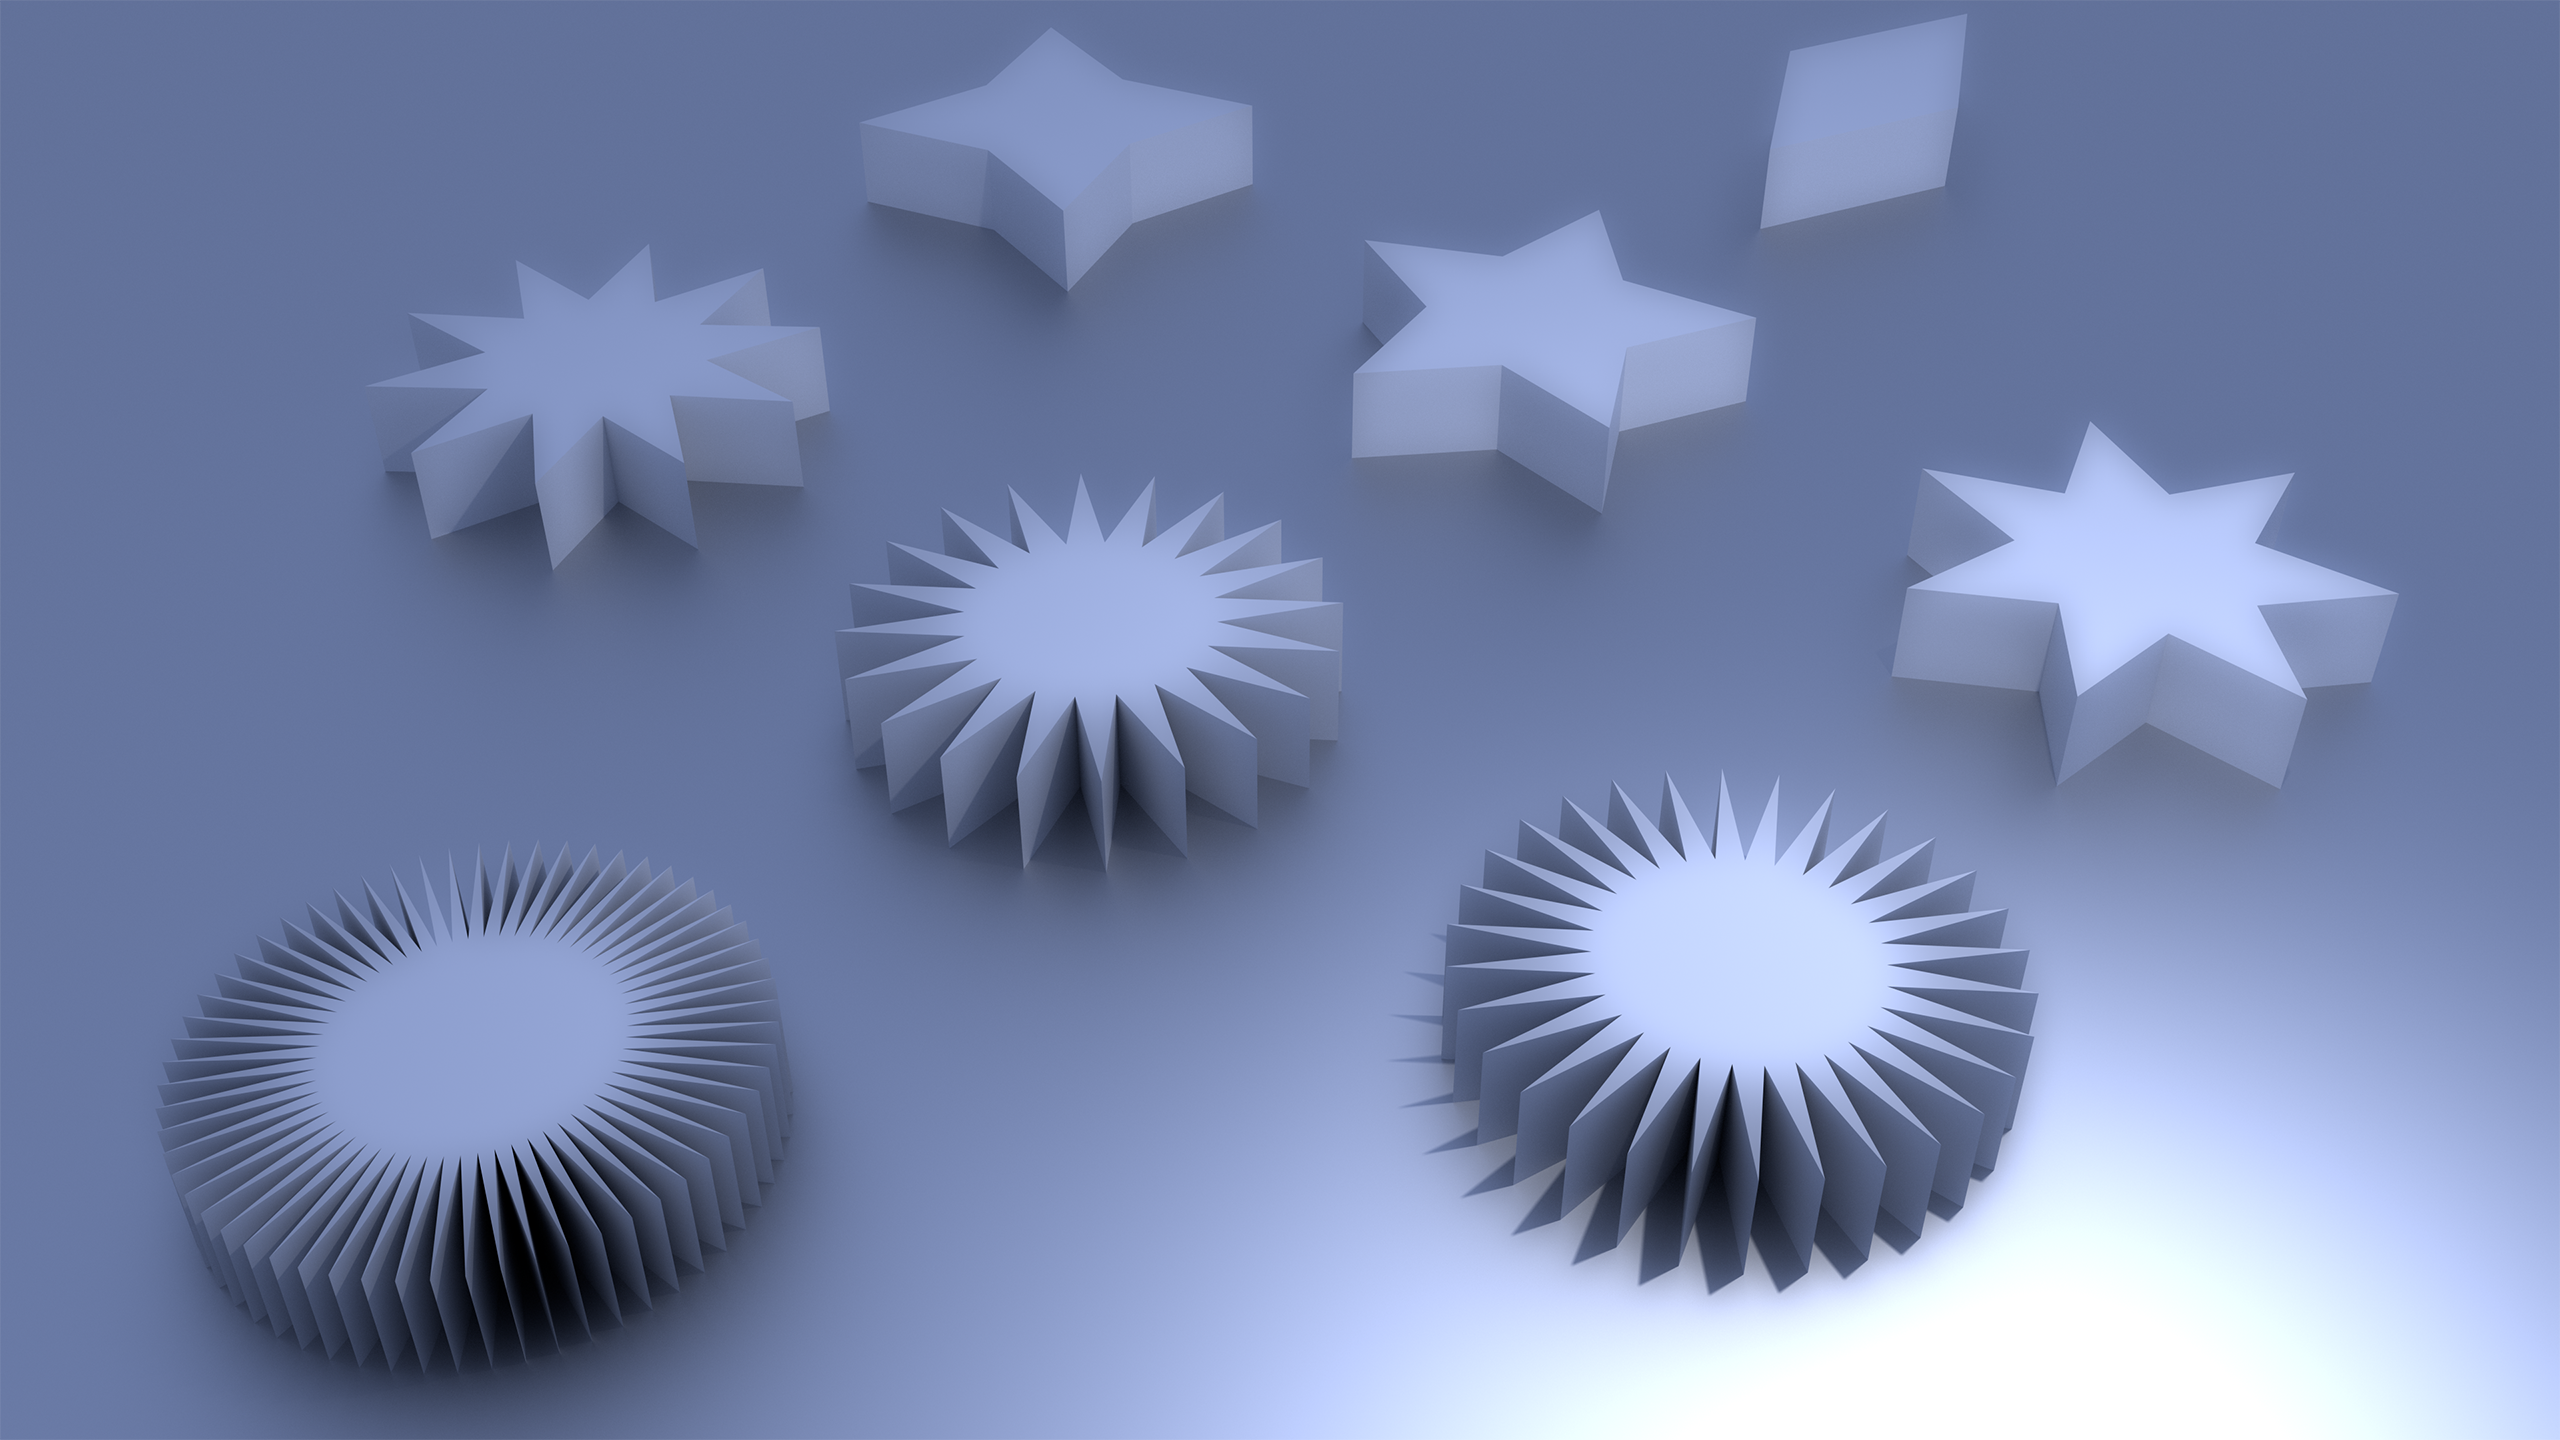
\includegraphics[width=.44\textwidth]{entwurf/star_2-4-5-7-10-20-30-60}}
				{\caption{Gute Unterscheidung von vorn}\label{fig:formen:sterne3d:front}}%
		\end{subfloatrow}
		\hspace*{\columnsep}%
		\begin{subfloatrow}
		\hsize0.7\hsize
		\vbox {%
			\ffigbox[\FBwidth][\FBheight]
				{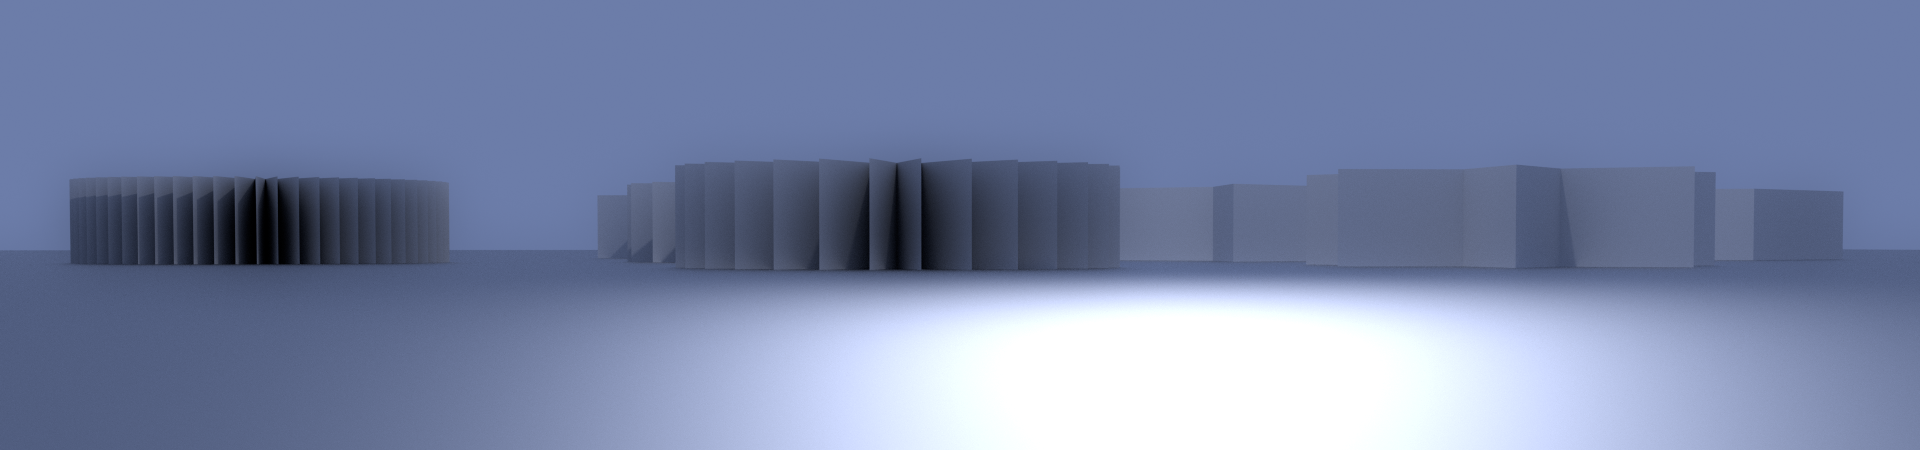
\includegraphics[width=.41\textwidth]{entwurf/star_2-4-5-7-10-20-30-60-seite}}
				{\caption{Die Unterschiede von der Seite \ldots}\label{fig:formen:sterne3d:side}}\vss
			\ffigbox[\FBwidth][\FBheight]
				{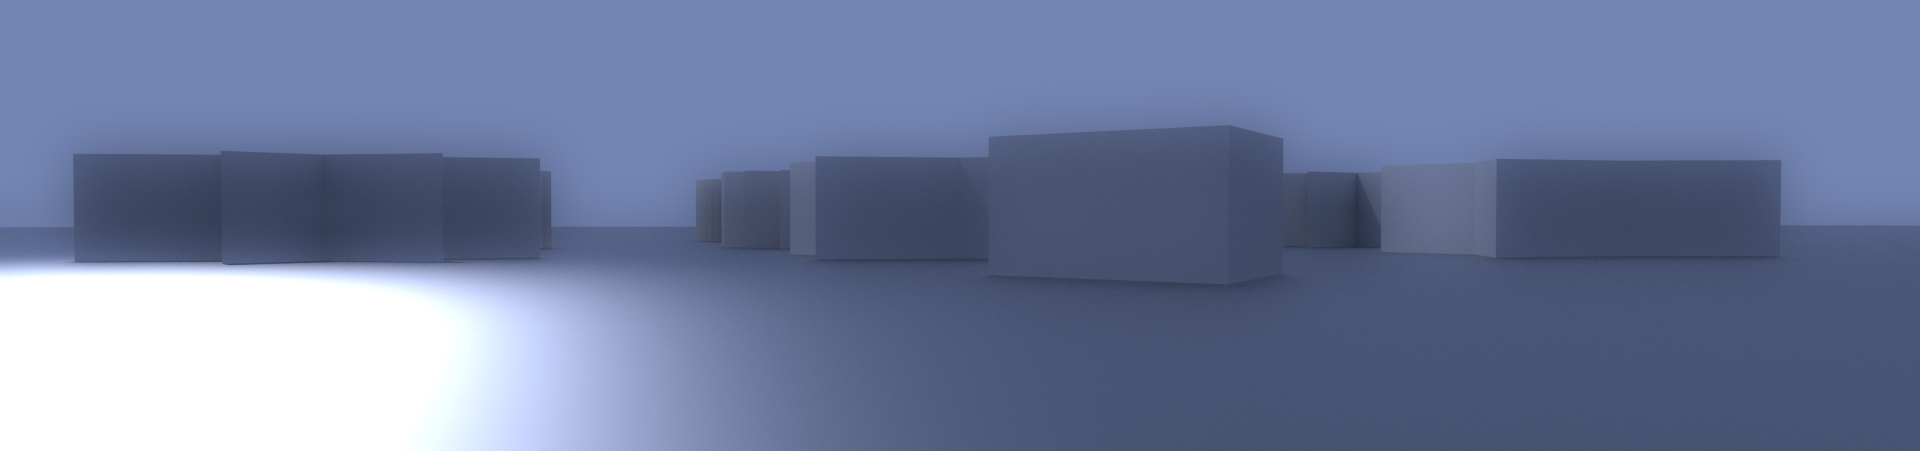
\includegraphics[width=.41\textwidth]{entwurf/star_2-4-5-7-10-20-30-60-oben}}
				{\caption{\ldots bzw. von oben sind kleiner.}\label{fig:formen:sterne3d:top}}
		}
		\end{subfloatrow}
	}
	{\caption{Formgebung mit sternenförmigem, nichtkonvexen Prisma. ERKENNBARKEIT SCHLECHTER ALS BEI TRANS UNTEN?}\label{fig:formen:sterne3d}}
\end{figure}

\begin{figure}
	\ffigbox[\FBwidth] {
		\begin{subfloatrow}
			\ffigbox[\FBwidth][]
			{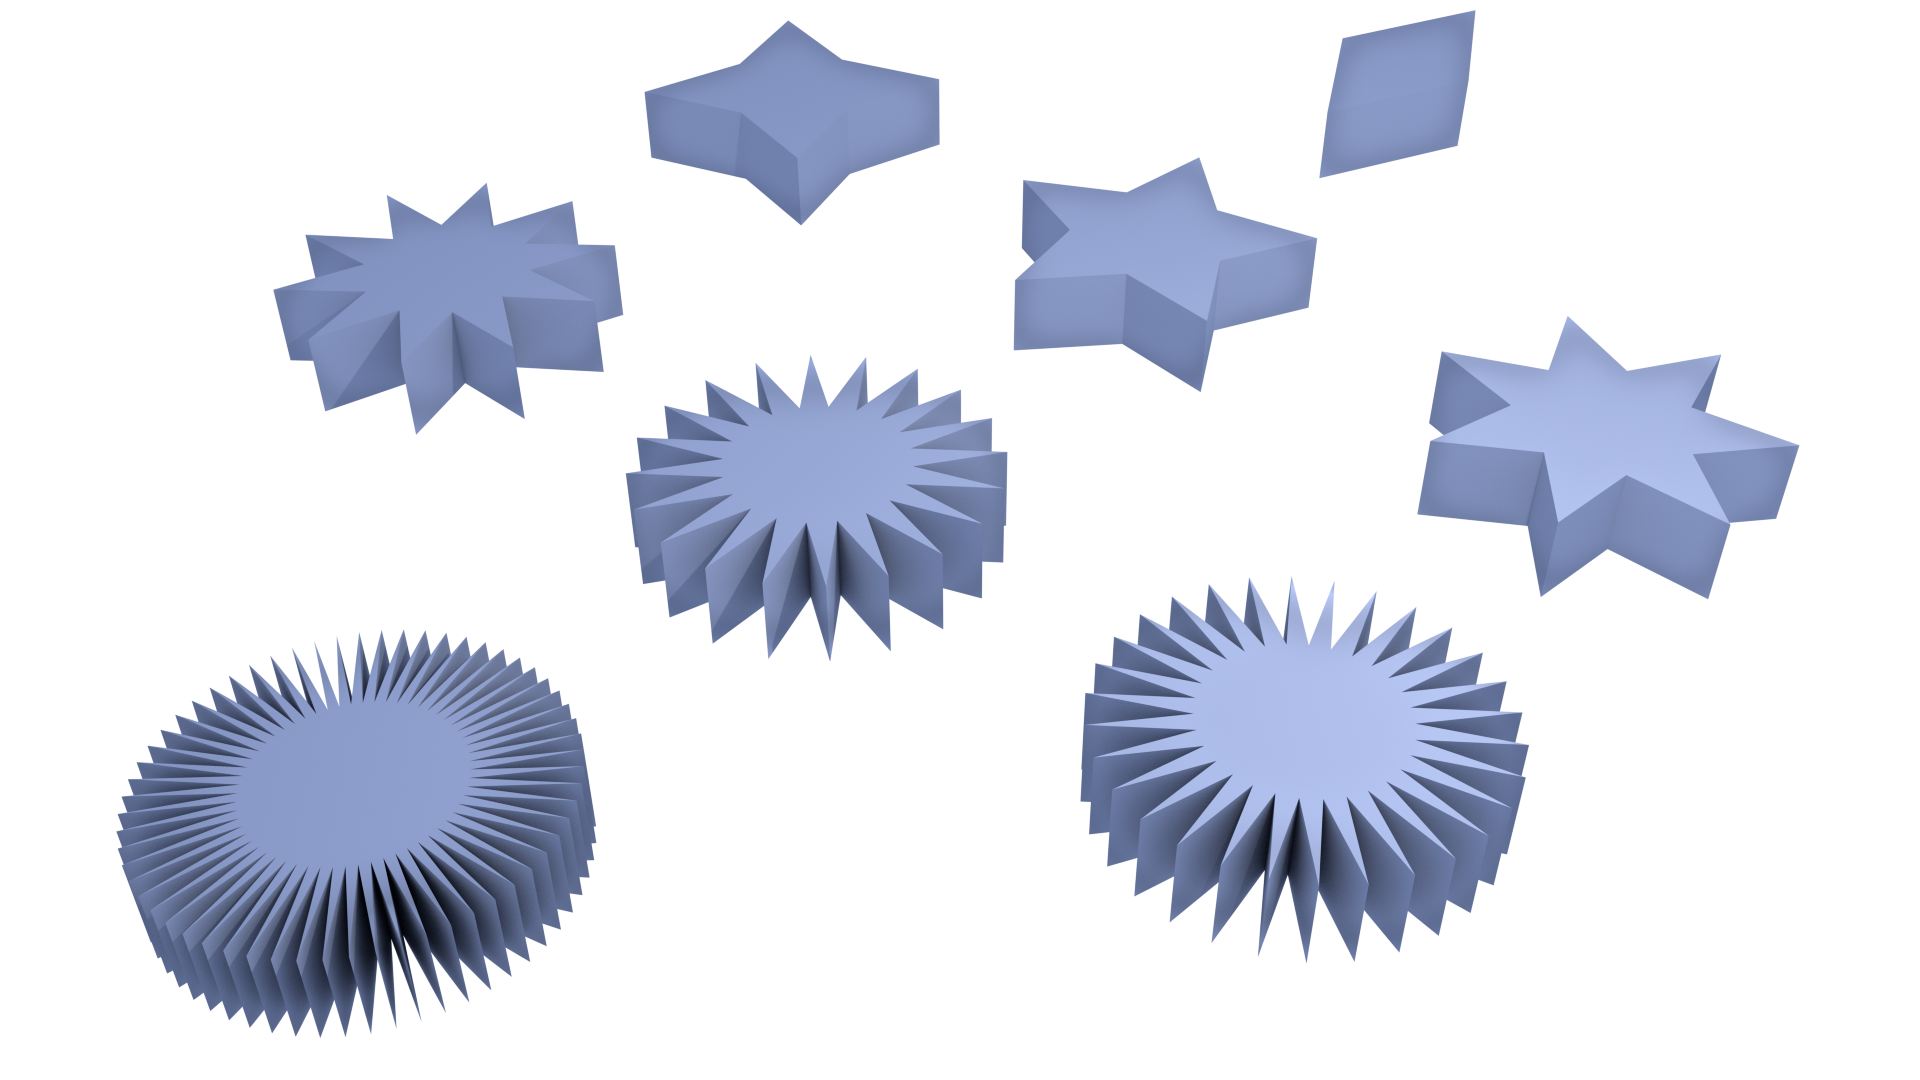
\includegraphics[width=.44\textwidth]{entwurf/star_2-4-5-7-10-20-30-60-trans}}
			{\caption{Gute Unterscheidung von vorn}\label{fig:formen:sterne3d:front-trans}}%
		\end{subfloatrow}
		\hspace*{\columnsep}%
		\begin{subfloatrow}
			\hsize0.7\hsize
			\vbox {%
				\ffigbox[\FBwidth][\FBheight]
				{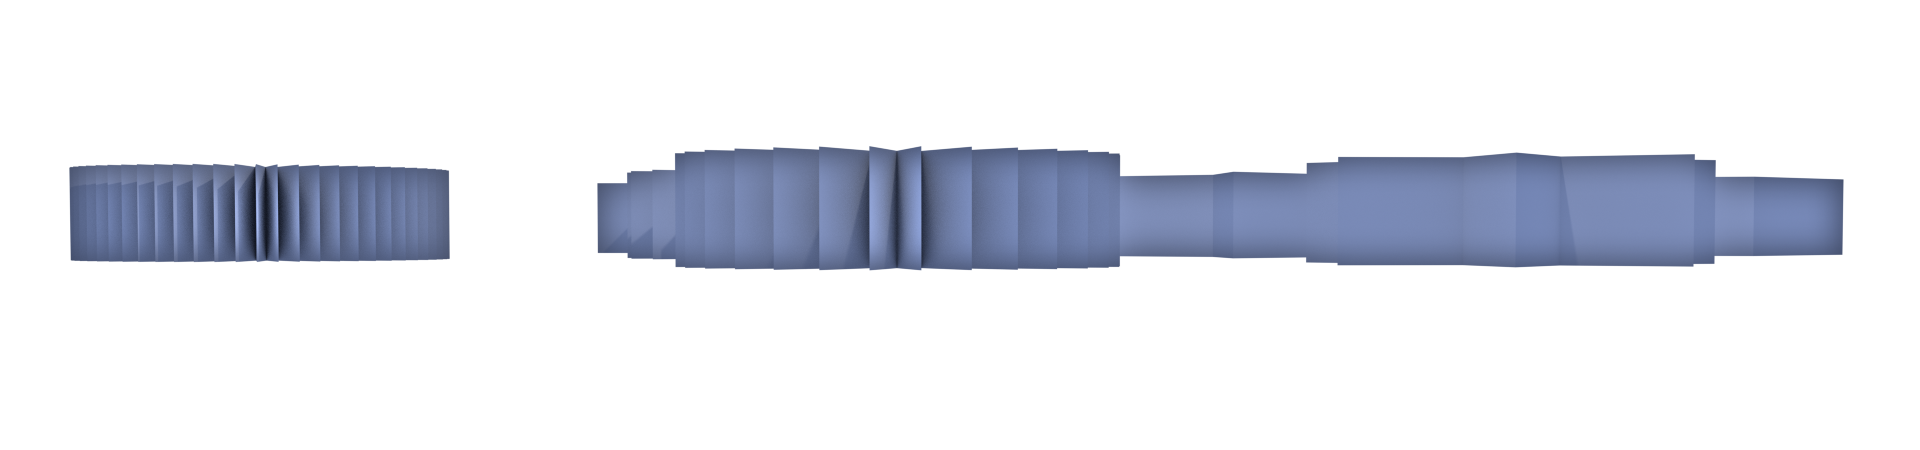
\includegraphics[width=.41\textwidth]{entwurf/star_2-4-5-7-10-20-30-60-seite-trans}}
				{\caption{Die Unterschiede von der Seite \ldots}\label{fig:formen:sterne3d:side-trans}}\vss
				\ffigbox[\FBwidth][\FBheight]
				{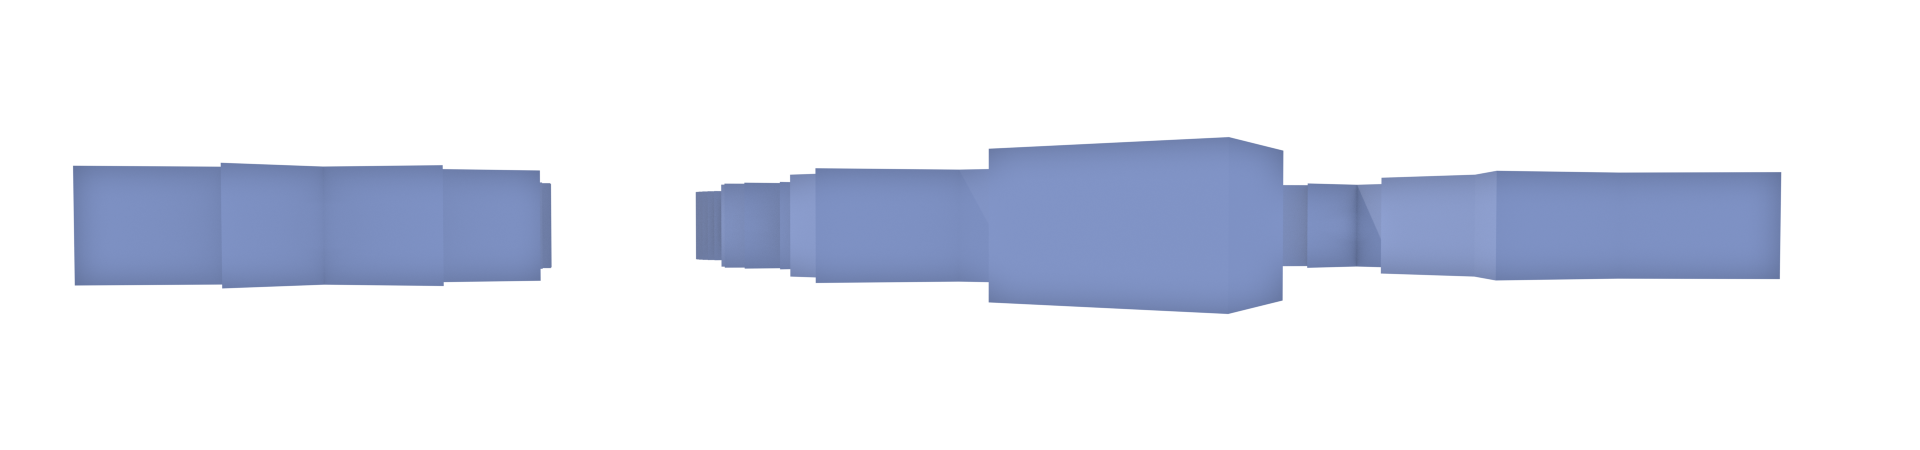
\includegraphics[width=.41\textwidth]{entwurf/star_2-4-5-7-10-20-30-60-oben-trans}}
				{\caption{\ldots bzw. von oben sind kleiner.}\label{fig:formen:sterne3d:top-trans}}
			}
		\end{subfloatrow}
	}
	{\caption{Formgebung mit sternenförmigem, nichtkonvexen Prisma. TRANSPARENT}\label{fig:formen:sterne3d-trans}}
\end{figure}

Die Anforderung, eine Formgebung zu wählen, die einen ähnlichen Umkugelradius und damit eine einheitliche Größe erhält, einen aus allen Winkeln ähnlichen Durchmesser sowie eine ähnliche Form aufweist, führt zu bestimmten Gruppen von Polyedern. Polyeder sind dreidimensionale Polytope und im engeren Sinne eine Teilmenge des \gls{3dRaum}, welche ausschließlich durch gerade Flächen begrenzt wird. Darunter zählen unter anderem die fünf \propernames{platonischen}{platonischer Körper} \cite{RegularPolyhedra}, die 13 \propernames{archimedischen}{archimedischer Körper}, die 13 \propernames{catalanischen}{catalanischer Körper} sowie die 92 \propername{Johnson-Körper} \cite{JohnsonPolyeder}. Eine Charakteristik dieser Polyeder ist ihre konvexe Form, was gleichzeitig die Unterscheidung aus der Distanz erschwert. Die prismatischen Polyeder fallen ebenfalls unter diese Kategorie, werden jedoch aus denselben Gründen ausgeschlossen wie die sternenförmigen Prismen.

Andererseits erfüllen die sternförmigen \propername{Kepler-Poinsot-Körper} (,,Sternpolyeder'') die Anforderungen. Sie besitzen im Gegensatz zu den vorgenannten Polyedern auch konkave Flächen \cite{KeplerPoinsotSolid} und können daher, wie in der interaktiven Visualisierung von \cite{WebGLUniformPolyhedra} zu sehen, leicht von den konvexen Polyedern unterschieden werden.

Ebenfalls geeignet ist der Vorschlag, eine Sternform durch sogenanntes \textquote{Poken} zu erzeugen: \blockcquote[4]{ProceduralGenerationofSculpturalForms}{By “poke” we mean a function to create a pyramid on each face of a given object. (This is different from Kepler’s stellation operation, which extends the face planes.)}

Somit gibt es mit der auf nichtprismatischen Polyedern basierenden Formgebung eine hohe Anzahl verschiedener Formen, die alle die Anforderung an eine einheitliche Größe, an einen aus allen Blickwinkeln ähnlichen Durchmesser und an die Wiedererkennbarkeit gewährleisten. Lediglich die Unterscheidung innerhalb der konvexen Polyeder kann schwerfallen. Am Deutlichsten unterscheiden sich die \propernames{platonischen Körper}{platonischer Körper} untereinander sowie die konvexen von den konkaven, sternförmigen Polyedern.

\chapter{MegaMol}

\section{Daten}
Beim Laden beider mmpld (default und signed distance) kommt der Fehler R6010: abort() has been called, trotz unbegrenzter Speichereinstellung bei MMPLDDataSource. Es wurden maximal 20 Zeitschritte jeweils geladen (SplitView) bzw. maximal 40 (SingleView) - wegen 32bit (max 1,7GiB RAM Zuweisung wurden angezeigt)! Ein Wechsel auf 64bit hat geholfen (8GiB Arbeitsspeicher noch zu wenig).

\section{Modules}
\begin{itemize}
\item Callee: Eingänge, angesprochen über ihre Descriptions
\item Caller: Ausgänge
\end{itemize}

Die verfügbaren Module sind je nach Callee/Callertyp unterschiedlich. Beispiele für Typen sind CallGetTransferFunction, MultiParticleDataCall, CallRenderView oder CallRender3D, einstellbar bei der Definition der Callbackfunktion für den Callee/Caller. Diese werden über die Descriptions der Typen angesprochen:
\begin{lstlisting}[language=c]
typedef factories::CallAutoDescription
\end{lstlisting}

Modifikationen von Eigenschaften von Elementen in anderen Modulen werden über den Callee/Callertyp übermittelt, z.B.

\begin{lstlisting}[language=c]
core::view::CallGetTransferFunction *cgtf = dynamic_cast<core::view::CallGetTransferFunction*>(&call);
// [...]
cgtf->SetTexture(this->texID, this->texSize, this->texFormat);
\end{lstlisting}

Zugriff auf die einzelnen Partikel einer MMPLD: megamol::core::moldyn::MultiParticleDataCall

\chapter{Visualisierungsentwurf}

\section{Taxonomie der Visualisierung}
Die Berechnung des Clusterverhaltens ergibt eine Datenbank, in der Ereignisse abgelegt sind. Ein Ereignis stellt einen Datensatz dieser Datenbank dar, die Parameter des Ereignisses sind die Datensatzfelder. Die Aufgabe der Visualisierung ist es, den Parametern eines Ereignisses visuelle Attribute zuzuweisen. Diese Zuweisung kann in einer weiteren Datenbank als Relation %im Sinne des \gls{rdbms}
zwischen Parameter und Attribut festgehalten werden.

Zum leichteren Verständnis erfolgt eine Einteilung der Parameter, der Attribute sowie der Zuweisungen in die beiden in \autoref{fig:entwurf:taxonomie:vartype} gezeigten Variablentypen. Der Typ \propername{Zahlenwert} steht dabei für die Nutzung eines kontinuierlichen Zahlenraumes, während der Variablentyp \propername{Vokabular} eine diskrete, beschränkte Zuordnung mit voneinander disjunkten Elementen beschreibt.

\begin{figure}
	\begin{tikzpicture}[]
		\node {Variablentyen im Entwurf}
		child { node [value] {Zahlenwert} }
		child { node [vocab] {Vokabular} };
	\end{tikzpicture}
	\caption{Taxonomie der Variablentypen}\label{fig:entwurf:taxonomie:vartype}
\end{figure}

\subsection{Parameter eines Ereignisses}
Ein Ereignis besteht aus drei Parametern, die jeweils zwischen ein bis drei Freiheitsgraden aufweisen.

\begin{itemize}
	\item Zeitpunkt: ein Wert (t)
	\item Ort: drei Werte (x, y, z)
	\item Art: ein Vokabular [Split, Merge, Death, Birth]
\end{itemize}

\subsection{Visuelle Attribute eines Ereigniselements}\label{sec:attribute}
Die visuellen Attribute können sowohl als fließender \propername{Zahlenwert} als auch als festes \propername{Vokabular} umgesetzt werden. Beispielsweise bedeutet der Vokabulartyp für das \visattrs{Positionsattribut}{Position} die Festlegung bestimmter Koordinaten für jeden Begriff des Vokabulars.

Jedes Attribut besitzt eine individuelle Anzahl an Freiheitsgraden, die zur Visualisierung genutzt werden können.

\begin{itemize}
	\item Position: 3 (x, y, z)
	\item Farbe: 2 (Farbwert/Sättigung, Helligkeit)
	\item Form: 1, eine Wertzuweisung ist möglich durch die Anzahl der Ecken, Kanten und Flächen. Anderes wie z.B. der Abstand der Ecken vom Körperzentrum kollidiert mit dem Attribut Größe.
	\item Größe: 1
	\item Opazität: 1
\end{itemize}

Da Farbwerte bei geringer Sättigung nicht mehr voneinander unterschieden werden können, werden diese beiden Farbeigenschaften zusammengefasst. Dadurch kann die Helligkeit leicht als separates Attribut vom Betrachter erkannt werden, wie in \autoref{fig:entwurf:farbtafel} zu sehen.

\begin{figure}
	VERGLEICHSBILD MIT WECHSELNDER SÄTTIGUNG UND HELLIGKEIT
	%\includegraphics[width=.8\textwidth]{entwurf/}
	\caption{Farbtafel mit unterschiedlicher Sättigung und Helligkeit}\label{fig:entwurf:farbtafel}
\end{figure}

Bei der \visattr{Form} sind mehrere Freiheitsgrade möglich, etwa eine Kombination aus Anzahl der Ecken mit einem variablen Abstand dieser vom Körperzentrum. Der variable Abstand kollidiert jedoch mit dem Attribut \visattr{Größe}. Daher wird das Attribut \visattr{Form} auf einen Freiheitsgrad beschränkt und es werden die in \autoref{sec:grundlagen:formgebung} beschriebenen Polyeder verwendet. Da die Anzahl an Polyedern begrenzt ist und die Unterscheidungsmöglichkeit mit zunehmender Flächenanzahl sinkt, ist das Attribut \visattr{Form} nur eingeschränkt als Zahlenwert verwendbar.

Bei der Bestimmung der Attribute wurde darauf geachtet, ein umfassendes Spektrum der Gestaltgesetze nutzen zu können. Alle visuellen Attribute fallen unter den Einfluss des \viss{Gesetzes der Prägnanz}{Gesetz der Prägnanz}. Mit der \visattr{Position} kann das \vis{Gesetz der Nähe} sowie das \vis{Gesetz der gemeinsamen Region} genutzt werden, eine Kombination aus der \visattr{Position} mit den anderen Attributen resultiert in der Verwendbarkeit des \viss{Gesetzes der Kontinuität}{Gesetz der Kontinuität}. Bis auf die \visattr{Position} kann mit allen visuellen Attributen das \vis{Gesetz der Ähnlichkeit} genutzt werden. Das \vis{Gesetz der Geschlossenheit} kann mit dem \visattrs{Positionsattributs}{Position} verarbeitet werden, falls durch entsprechende Zuweisung die Elemente nah beieinander lägen und sie eine geschlossene Form bilden. Mit den hier definierten Attributen kann somit von sechs der zehn in \autoref{sec:gestaltgesetze} aufgezählten Gestaltgesetze Gebrauch gemacht werden.

Texturen als ein eigenständiges visuelles Attribut werden ausgeklammert, da sie sich mit dem Attribut \visattr{Farbe} und bei der Nutzung als Oberflächenstruktur mit dem Attribut \visattr{Form} überschneiden. Ein Einsatz als Bump Map oder Displacement Map zur Unterstützung des Attributs \visattr{Form} wäre denkbar. Aufgrund dessen, dass bereit Polyeder für das \visattrs{Formattribut}{Form} genutzt werden, wird von einer Verwendung von Texturen allerdings abgesehen.

Animationen bieten weitere visuelle Attribute wie Bewegungsrichtung, Bewegungsbahn, Beschleunigung und Geschwindigkeit als auch die Veränderung der anderen Attribute und eröffnen damit die Nutzung des \viss{Gesetzes der Gleichzeitigkeit}{Gesetz der Gleichzeitigkeit} sowie des \viss{Gesetzes der gemeinsamen Bewegung}{Gesetz der gemeinsamen Bewegung}. Sie werden im Rahmen dieser Arbeit jedoch nicht behandelt.

Die visuellen Attribute lassen sich durch den Betrachter unterschiedlich gut unterscheiden. In der folgenden Sortierung nach ihrer Unterscheidungsgüte stehen die am Leichtesten zu unterscheidenden Attribute ganz oben. (QUELLE)
\begin{enumerate}
	\item Position
	\item Farbwert
	\item Größe
	\item Form
	\item Helligkeit
	\item Opazität
\end{enumerate}

Die Attribute mit höherer Unterscheidungsgüte sollten bevorzugt gewählt werden. Form, Helligkeit und Opazität sind durch die geringere Güte besser als Vokabular- denn als Wertattribut geeignet, da bei den Vokabularen die Anzahl der Begriffe im Vergleich zur Menge der Zahlenwerte gering ist. Dadurch können die Attributseigenschaften weiter auseinanderliegen, was eine leichtere Unterscheidung ermöglicht.

Die 

In der \tool{MegaMol} Molekularsimulation wird ausschließlich das visuelle Attribut \visattr{Position} zur Darstellung genutzt.

\begin{figure}
	\ffigbox[\FBwidth] {
		\begin{subfloatrow}
			\ffigbox[\FBwidth] {
				\fbox {
					\begin{tikzpicture}[level 1/.style={sibling distance=1.4cm}]
					\node {Ereignis}
					child { node [value] {Zeitpunkt} }
					child { node {Ort}
						child [verticalChild, first] { node [value] {x} }
						child [verticalChild, second] { node [value] {y} }
						child [verticalChild, third] { node [value] {z} }
					}
					child { node [vocab] {Art}
						child [verticalChild, first] { node {Split} }
						child [verticalChild, second] { node {Merge} }
						child [verticalChild, third] { node {Death} }
						child [verticalChild, fourth] { node {Birth} }
					};
					\end{tikzpicture}
				}
			}
			{\caption{Ereignis mit Variablentyp}\label{fig:entwurf:taxonomie:ereignis}}%
			
			\ffigbox[\FBwidth] {
				\fbox {
					\begin{tikzpicture}[level 1/.style={sibling distance=1.8cm}]
					\node {Visuelles Attribut}
					child { node {Position}
						child [verticalChild, first] { node [] {x} }
						child [verticalChild, second] { node [] {y} }
						child [verticalChild, third] { node [] {z} }
					}
					child { node {Farbe}
						child [verticalChild, first] { node [] {Farbwert \& S"attigung} }
						child [verticalChild, second] { node [] {Helligkeit} }
					}
					child { node [] {Größe} }
					child { node [] {Form}	}
					child { node [] {Opazität} }
					;
					\end{tikzpicture}
				}
			}
			{\caption{Die visuellen Attribute können beide Variablentypen annehmen.}\label{fig:entwurf:taxonomie:variable}}
		\end{subfloatrow}
	}
	{\caption{Taxonomie der Daten und visuellen Attribute}\label{fig:entwurf:taxonomie}}
\end{figure}

\subsection{Problem der lokalen und temporalen Agglomeration}\label{sec:entwurf:agglomeration}

Die Anzahl der Datensätze, die denselben Ort oder denselben Zeitpunkt aufweisen können, ist unbekannt. Schon eine geringe Anzahl identischer Orte oder Zeitpunkte kann je nach Zuordnung der visuellen Attribute zu einer überlagerten, nicht mehr unterscheidbaren Darstellung führen, wodurch die Erkennung solcher Agglomerate nicht gegeben ist. Daher wird ein visuelles Attribut reserviert, um eine solche Anhäufung von Ereignissen anzuzeigen. Die \dataparam{Häufung} wird bei der Zuweisung zu den visuellen Attributen wie ein Ereignisparameter behandelt. Abhängig von dieser Zuweisung in \autoref{sec:entwurf:zuweisung:parameter-attribut} können zwei Werte für die lokale und temporale Häufigkeit notwendig sein. Dieser wird jedem Ereignis zugewiesen und wird beim Auffinden von identischen Ortsparametern bzw. Zeitparametern in den Datensätzen inkrementiert.

Die Begriffe \dataparam{Agglomeration} und \dataparam{Häufung} sind hier synonym.

Bei der Visualisierung von Agglomeraten kann die natürliche Wirkung (QUELLE) der visuellen Attribute genutzt werden. Groß, opaque und dunkel stehen für eine starke Agglomeration. Klein, transparent und hell für eine niedrige.

\subsection{Verbundenheit}\label{sec:entwurf:verbundenheit}
Wenn sich ein Cluster teilt (Split) und sich die resultierenden Cluster wiederrum teilen oder mit anderen Clustern verschmelzen (Merge), so kann man diesen Ereignissen Vorgänger (Eltern) sowie Nachfolger (Kinder) zuordnen. IST DAS RICHTIG?

\vis{Gesetz der Geschlossenheit}
\vis{Gesetz der fortgesetzt durchgehenden Linie}
\vis{Gesetz der verbundenen Elemente}


\section{Parameter-Attributszuweisung}\label{sec:entwurf:zuweisung:parameter-attribut}

In der \propername{MegalMol} Simulation wird der Ort des Ereignisses mithilfe der Teilchenposition dynamisch visualisiert. Insofern kann angenommen werden, dass für eine nahtlose Benutzbarkeit zwischen der \tool{MegaMol} Animation und der statischen Visualisierung die Zuweisung des Elementattributes \visattr{Position} an den Parameter \dataparam{Ort} empfehlenswert ist. Weiterhin ist die Reservierung der \visattr{Opazität} für die \dataparam{Häufung} die einfachste Möglichkeit, denn dies hat zwei Vorteile. Zum Einen ist keine nachträgliche Modifizierung der visuellen Attribute der einzelnen Ereignisse notwendig, denn die Opazitätseigenschaft sorgt durch Überlagerung für eine von der Anzahl direkt abhängige Hintergrundverdeckung. Dadurch werden zum Anderen auch keine Informationen über die Häufigkeit im Datensatz benötigt. Hingegen muss zum Beispiel eine Größenveränderung nachträglich für jedes Ereignis im Agglomerat auf der Basis eines temporalen oder lokalen \dataparams{Häufungswert}{Häufung} durchgeführt werden.

Darüberhinaus wird jedem Ereignisparameter nur eine visuelles Attribut zugeordnet, denn Mehrfachzuweisungen sollten wegen einer Verminderung der präattentiven Wahrnehmung (VERWEIS AUF GRUNDLAGEN) vermieden werden.

Daraus ergeben sich die in \autoref{tab:entwurf:zuweisung-param-attr:position-agglo} aufgeführten Visualisierungsmöglichkeiten.

\begin{table} 
	\begin{tabularx}{\textwidth}{@{}CCCCCCCCC@{}}
		\toprule
		Attribute & Position x & Position y & Position z & Farbwert \& Sättigung & Helligkeit & Eckenanzahl & Größe & Opazität \tabularnewline
		\midrule
		& Ort x & Ort y & Ort z & Art & Zeit & & & H \tabularnewline
		& Ort x & Ort y & Ort z & Art & & Zeit & & H \tabularnewline 
		& Ort x & Ort y & Ort z & Art & & & Zeit & H \tabularnewline 
		& Ort x & Ort y & Ort z & Art & & & & H \tabularnewline 
		\midrule
		& Ort x & Ort y & Ort z & Zeit & Art & & & H \tabularnewline 
		& Ort x & Ort y & Ort z & & Art & Zeit & & H \tabularnewline
		& Ort x & Ort y & Ort z & & Art & & Zeit & H \tabularnewline 
		& Ort x & Ort y & Ort z & & Art & & & H \tabularnewline 
		\midrule
		& Ort x & Ort y & Ort z & Zeit & & Art & & H \tabularnewline 
		& Ort x & Ort y & Ort z & & Zeit & Art & & H \tabularnewline 
		& Ort x & Ort y & Ort z & & & Art & Zeit & H  \tabularnewline
		& Ort x & Ort y & Ort z & & & Art & & H  \tabularnewline
		\midrule
		& Ort x & Ort y & Ort z & Zeit & & & Art & H \tabularnewline 
		& Ort x & Ort y & Ort z & & Zeit & & Art & H \tabularnewline 
		& Ort x & Ort y & Ort z & & & Zeit & Art & H \tabularnewline 
		& Ort x & Ort y & Ort z & & & & Art & H \tabularnewline 
		\bottomrule
	\end{tabularx}
	\caption{Zuweisungsmöglichkeiten der Parameter zu den visuellen Attributen bei Kopplung des \dataparams{Ortes}{Ort} an die \visattr{Position}. Zur Anzeige der Häufung H wird die \visattr{Opazität} reserviert. Die Zeit wird in einigen Varianten nicht kodiert.}\label{tab:entwurf:zuweisung-param-attr:position-agglo}
\end{table}

Derzeit ist nicht bekannt, wie groß die örtliche Konzentration von Ereignissen ist. Sollte sie eine kritische Anzahl überschreiten und das der \dataparam{Häufung} zugewiesene Attribut keine sinnvollen Ergebnisse mehr liefern können, so kann der Ort des Ereignisses einem anderen Attribut zugewiesen werden. Weiterhin kann das Loslösen des \dataparams{Ortes}{Ort} von der Position sinnvoll sein, wenn für eine Auswertung der Ort des Ereignisses nur eine untergeordnete Rolle spielt. Vorschläge für entsprechende Zuweisungsmöglichkeiten sind in \autoref{tab:entwurf:zuweisung-param-attr:frei} zu finden.

\begin{table}
	\begin{tabularx}{\textwidth}{@{}CCCCCCCCC@{}}
		\toprule
		Attribute & Position x & Position y & Position z & Farbwert \& Sättigung & Helligkeit & Eckenanzahl & Größe & Opazität \tabularnewline
		\midrule
		& Zeit & H & & Art \tabularnewline
		& Zeit & Art & & H & Ort x \tabularnewline
		& Ort x & Art & & & & & H \tabularnewline
		& Ort x & Zeit & & & & H & \tabularnewline
		\bottomrule
	\end{tabularx}
	\caption{Ausgewählte Zuweisungsmöglichkeiten der Parameter zu den visuellen Attributen bei Loslösung des \dataparams{Ortes}{Ort} von der \visattr{Position} sowie Trennung der \dataparam{Häufung} H von der \visattr{Opazität}. Nicht jeder Parameter wird kodiert. UNVOLLSTÄNDIG}\label{tab:entwurf:zuweisung-param-attr:frei}
\end{table}

Da jedoch in der Molekularsimulation der Ort eines Ereignisses der visuellen Position zugewiesen ist und die Visualisierung in der vorliegenden, ersten Iteration mit der Simulation harmonieren soll, erfolgt die Zuweisung des Ortes ausschließlich an die \visattr{Position}, so dass die weitere Betrachtung auf die in \autoref{tab:entwurf:zuweisung-param-attr:position-agglo} gezeigten Zuweisungsmöglichkeiten beschränkt wird.

\section{Mockups}\label{sec:mockups}

\subsection{Werkzeug}\label{sec:mockups:werkzeug}
Zur Überprüfung einer sinnvollen Zuweisung der Parameter zu den Attributen dienen Mockups. Aufgrund der Vielzahl der in \autoref{sec:entwurf:zuweisung:parameter-attribut} genannten Kombinationsmöglichkeiten wird eine programmatische Erstellung der Mockups gewählt. Da eine schnelle Umsetzbarkeit im Vordergrund steht, wird \propername{Unity3D} als Entwicklungsumgebung gewählt. Ein Vorteil dieser Engine ist die Möglichkeit, rasch Prototypen erstellen zu können sowie die einfache Umsetzbarkeit für verschiedenste Plattformen, ohne auf Containermanager wie \href{https://www.docker.com/}{Docker} angewiesen zu sein. Letzterer Umstand ist für den möglichen Einsatz der Mockups als Evaluationswerkzeug von Bedeutung. Die Performance spielt beim Mockup eine untergeordnete Rolle.

Beim Deploy der \tool{Unity3D} WebGL Anwendung kam es auf bestimmten Apachekonfigurationen zu Problemen. Dies war durch eine \href{http://forum.unity3d.com/threads/html-mem-causes-http-500-internal-server-error-on-apache.309762/}{manuelle Umbenennung von Dateien und Verweisen} in der durch \tool{Unity3D} generierten Anwendung zu lösen. Von offizieller Seite wurde dies \href{http://forum.unity3d.com/threads/html-mem-causes-http-500-internal-server-error-on-apache.309762/#post-2014787}{als Bug markiert}. SOLCHE SÄTZE HABEN IN DER BA VERMUTLICH NIX ZU SUCHEN?

\subsection{Datensatz}\label{sec:mockups:daten}
Um eine Vergleichbarkeit der verschiedenen Mockups zu gewährleisten, liegt ein fester Datensatz in \autoref{tab:entwurf:mockup-data} zugrunde. Sämtliche Werte sind einheitenlos und wurden für die Parameter \dataparam{Ort} und \dataparam{Zeit} so gewählt, dass eine Überlappung der Ereigniselemente von nebeneinanderliegenden Ereignissen bei einer Zuweisung an das visuelle Attribut \visattr{Position} nicht auftritt, da andernfalls durch das \vis{Gesetz der verbundenen Elemente} ein falsches Abbild der zugrundeliegenden Daten übertragen werden würde. Der Zahlenbereich für die Zeit ist auf das Intervall $[1,22]$ begrenzt. Da sich in der Simulation die meisten Elemente mit zunehmender Zeit vom Zentrum entfernen, wird die $x$-Koordinate des Ortes mit \autoref{eq:mockup:zeit-ortx} direkt an die Zeit $t$ gekoppelt.
\begin{align}\label{eq:mockup:zeit-ortx}
	x = \left\lfloor\frac 43\cdot t + 0,5\right\rfloor
\end{align}
Aufgrund des zylinderförmigen Raumes in der Simulation wird sowohl für die $y$-Koordinate als auch für die $z$-Koordinate des Ortes ein identisches und kleineres Intervall von $[1,10]$ gewählt.

Die Zuweisung der \dataparam{Art} des Ereignisses erfolgt manuell. Da die simulierten Partikel in der \tool{MegaMol} zu Beginn der Simulation einen einzigen Cluster in flüssiger Phase bilden, kommen bei kleinen Zeitwerten vor allem Splits vor.

Zur Darstellung der in \autoref{sec:entwurf:agglomeration} beschriebenen Häufung, werden die Ereignisse $6-9$, $35/36$ sowie $46-48$ jeweils gruppiert und händisch an denselben Ort und dieselbe Zeit gesetzt.


\subsection{Zuweisung der Zahlenwerte}
Zur Gewährleistung der in \autoref{sec:mockups:daten} beschriebenen Vermeidung unnötiger Überlappungen der Ereigniselemente wird der Standardwert des Attributs \visattr{Größe}, d.h. wenn das Attribut keinem Parameter zugewiesen ist, entsprechend skaliert. Um nah bei der Visualisierung der Molekularsimulation selbst zu bleiben, wird in den Mockups, die nicht das Attribut \visattr{Form} beinhalten, eine Kugel verwendet. 

Die Attribute in den Mockups weisen folgende Zahlenbereiche auf:
\begin{itemize}
	\item x-, y-, z-Position: $[-\infty, \infty]$, beim Parameter \dataparam{Ort} erfolgt eine direkte Zuweisung 
	\item Farbwert: $[0, 340]\degree$ bei $100\%$ Sättigung (\gls{hsb} Modell)
	\item Helligkeit $[40, 100]\%$, Standardwert $100\%$ (\gls{hsb}-Modell)
	\item Form: besitzt keinen Zahlenbereich, sondern beinhaltet verschiedene Formen von Polyedern sowie die Kugel als Standardwert
	\item Skalierung: $[0.25,2]$, Standardwert $1$
	\item Opazität: $[40, 100]\%$, Standardwert $100\%$
\end{itemize}
Die Mindesthelligkeit $b_{\text{min}}$ von $40\%$ dient dazu, um noch eine Farbwertunterscheidung treffen zu können, genauso wie die Mindestopazität von ebenfalls $40\%$. Der Maximalfarbwert $h_{\text{max}}$ von $340\degree$ wird festgelegt, um eine Unterscheidung zu den niedrigen Farbwerten zu erhalten.

Da die Grenzwerte der visuellen Attribute $a_{\text{min}}$ und $a_{\text{max}}$ aus \autoref{sec:mockups} bekannt sind und sich für die Parameter $p$ aus \autoref{tab:entwurf:mockup-data} ein minimaler und maximaler Wert $p_{\text{min}}$ und $p_{\text{max}}$ bestimmen lässt, wird für die Berechnung der Attributwerte die Linearfunktion in \autoref{eq:mockup-linearfunktion} verwendet.

\begin{equation}
\begin{aligned}\label{eq:mockup-linearfunktion}
a &= m \cdot p + n\\
a_{\text{max}} &= m \cdot p_{\text{max}} + n\\
a_{\text{min}} &= m \cdot p_{\text{min}} + n\\
m &= \boxed{\frac{a_{\text{max}} - n}{p_{\text{max}}}}\\
n &= a_{\text{min}} - m \cdot {p_{\text{min}}} = a_{\text{min}} - \frac{a_{\text{max}} - n}{p_{\text{max}}} \cdot p_{\text{min}}\\
&= a_{\text{min}} - a_{\text{max}} \cdot \frac {p_{\text{min}}}{p_{\text{max}}} + n \cdot \frac {p_{\text{min}}}{p_{\text{max}}}\\
n \cdot p_{\text{max}} &= a_{\text{min}} \cdot p_{\text{max}} - a_{\text{max}} \cdot p_{\text{min}} + n \cdot p_{\text{min}}\\
n \cdot \left( p_{\text{max}} - p_{\text{min}}\right) &= a_{\text{min}} \cdot p_{\text{max}} - a_{\text{max}} \cdot p_{\text{min}}\\
n &= \boxed{\frac{a_{\text{min}} \cdot p_{\text{max}} - a_{\text{max}} \cdot p_{\text{min}}}{p_{\text{max}} - p_{\text{min}}}}\\
\end{aligned}
\end{equation}

Anschließend erfolgt eine Rundung zur handlichen Verwendung der Ergebnisse.
\begin{align}\label{eq:mockup-rundung}
	a = \left\lfloor m \cdot p + n + 0,5 \right\rfloor
\end{align}

Die Berechnungsergebnisse sind in \autoref{sec:mockups:berechnungen} zu finden.

\subsection{Zuweisung des Vokabulars}

Da die Mächtigkeit $M$ des Vokabulars von \dataparam{Art} bekannt ist, kann das Intervall $v$ des Attributs $a$ in \autoref{eq:mockup-vokabular} zur rechnerischen Ermittlung der Attributwerte $a_i$ genutzt werden.

\begin{equation}
\begin{aligned}\label{eq:mockup-vokabular}
M &= 4\\
\Rightarrow p_{0\ldots 3} &= \left( 0, \frac 13, \frac 23, 1 \right) \\
v &= a_{\text{max}} - a_{\text{min}}\\
\\
a_i &= \left\lbrace p_i \cdot v + a_{\text{min}} \left| 0 \le i \le M-1 \right. \right\rbrace 
\end{aligned}
\end{equation}

Ausnahmen bilden die Attribute \visattr{Farbe} und \visattr{Form}. Wegen der kleinen Mächtigkeit des Vokabulars und zur Sicherung einer optimale Aufteilung des Farbwerts, wird dieser in \autoref{tab:entwurf:mockup-art} manuell definiert. Bei dem Attribut \visattr{Form} werden zur optimalen Unterscheidung vier Varianten aus der Menge der \propernames{platonischen Körper}{platonischer Körper} ausgewählt.

\begin{table}
	\begin{tabularx}{\textwidth}{@{}CRRRCR@{}}
		\toprule
		Art & Farbwert [°] & Helligkeit [\%] & Position x & Form & Größe \tabularnewline
		\midrule
		Death & 0   & 40  & 1  & T & 0,25 \tabularnewline
		Merge & 55  & 60  & 11 & H & 0,83 \tabularnewline
		Split & 245 & 80  & 21 & O & 1,42 \tabularnewline
		Birth & 145 & 100 & 31 & D & 2 \tabularnewline
		\bottomrule
	\end{tabularx}
	\caption{Festlegung der Attributeigenschaften für den Parameter \dataparam{Art} in den Mockups.}\label{tab:entwurf:mockup-art}
\end{table}

\subsection{Ausnahme: Konstanter Attributswert bei Opazität}

Aus den in \autoref{sec:entwurf:zuweisung:parameter-attribut} aufgeführten Gründen ist es sinnvoll, die \visattr{Opazität} der \dataparam{Häufung} zuzuweisen und sie mit einem konstanten Variablentyp auszustatten, so dass keine zusätzliche Ereigniswerte für die \dataparam{Agglomeration} benötigt werden. Dieser konstante Wert wird auf $50\%$ Opazität festgesetzt.

\subsection{Unterscheidbarkeit von Polyedern}

Da die Unterscheidung von Polyedern mit zunehmender Flächenanzahl schwieriger wird, findet im Mockup eine Begrenzung auf die fünf \propernames{platonischen Körper}{platonischer Körper} mit einer geringen Ecken- und Flächenanzahl statt.
\begin{description}
\item[T] Tetraeder mit 4 Ecken und 4 Flächen
\item[O] Oktaeder mit 6 Ecken und 8 Flächen
\item[H] Hexaeder mit 8 Ecken und 6 Flächen
\item[I] Icosaeder mit 12 Ecken und 20 Flächen
\item[D] Dodekaeder mit 20 Ecken und 12 Flächen
\end{description}
Die Abkürzungen folgen dem Vorschlag von Baierl \cite[S.~42]{KonvexePolyeder}. Bei der Modellierung in \tool{Blender} wurde für die Meshes die maximale Dimension von $1$ (einheitenlos) entsprechend der Dimension der kugelförmigen Standardelemente in \tool{Unity3D} gewählt.

\subsection{Verbundenheit}
Visuelle Relationen. Falls überhaupt möglich/benötigt (erstmal Ereignisse erstellen in MegaMol). Linien bieten sich an (Splines/Nurbs mal gucken).

NOCH NICHT IMPLEMENTIERT. WEITEREN DATENSATZ ERSTELLEN MIT ID'S AUS \autoref{tab:entwurf:mockup-data} mit der Struktur

\begin{lstlisting}[language=SQL]
/* MySQL */
CREATE TABLE relations (
	ID int NOT NULL AUTO_INCREMENT, /* int reicht fürs Mockup. */
	SourceID int NOT NULL,
	TargetID text NOT NULL, /* String, da unbekannte Anzahl an Targets. */
	PRIMARY KEY (ID)
	)
\end{lstlisting}

Alternativ Kinder/Eltern IDs für jedes Ereignis speichern.


\chapter{Entwurfsauswertung}

In den Abbildungen \autoref{fig:entwurf:frei} sind Beispiele dafür zu sehen, wenn die \dataparam{Häufung} anderen Attributen außer der \visattr{Opazität} zugewiesen wird.

\begin{figure}
	\caption{Mockups mit freier Positionszuweisung.}\label{fig:entwurf:frei}
\end{figure}

\chapter{Temporäre Notizen/Obsoletes}

\section{Alte Parameterattributszuweisung}

Aus den Parametern sowie der in \autoref{sec:attribute} genannten Qualität der Unterscheidungsmöglichkeit für die Attribute ergibt sich die in \autoref{tab:entwurf:attribute-zuweisungsart} aufgeführte Empfehlung.

\begin{table} 
	\begin{tabularx}{\textwidth}{@{}LCCC@{}}
		\toprule
		& Zeitpunkt & Ort & Art \tabularnewline
		\midrule
		Position & Wert & Wert & Vokabular \tabularnewline
		Größe & Wert & Wert & Vokabular \tabularnewline 
		Farbe & Wert & Wert & Vokabular \tabularnewline 
		Form & Vokabular & Vokabular & Vokabular \tabularnewline 
		Opazität & Wert & Wert & Vokabular \tabularnewline 
		\bottomrule
	\end{tabularx}
	\caption{Art der Zuweisung zwischen Parametern und Attributen}\label{tab:entwurf:attribute-zuweisungsart}
\end{table}


\begin{table}
	\begin{tabular}{l|ccc|c}
		& Zeitpunkt & Ort & Art (merge, split, death, birth) & örtliche und zeitliche Agglomeration \\
		\hline
		Position & \checkmark & \checkmark & \checkmark & \checkmark \\
		Größe & \checkmark & \kreuz & \checkmark & \checkmark \\
		Farbe & \checkmark & \kreuz & \checkmark & \checkmark \\
		Form & \kreuz & \kreuz & \checkmark & \checkmark \\
		Opazität & \checkmark & \kreuz & \checkmark & \checkmark \\
	\end{tabular}
	\caption{Matrix, was wie zusammenpasst und was nicht. Inzwischen überholt!}
\end{table}

\begin{table} 
	\begin{tabularx}{\textwidth}{@{}CCCCCCCCC@{}}
		\toprule
		Attribute & Position x & Position y & Position z & Farbwert \& Sättigung & Helligkeit & Eckenanzahl & Größe & Opazität \tabularnewline
		\midrule
		& Ort x & Ort y & Ort z & Art & Zeit \tabularnewline
		& Ort x & Ort y & Ort z & Art & & Zeit \tabularnewline 
		& Ort x & Ort y & Ort z & Art & & & Zeit \tabularnewline 
		& Ort x & Ort y & Ort z & Art & & & & Zeit \tabularnewline 
		\midrule
		& Ort x & Ort y & Ort z & Zeit & Art \tabularnewline 
		& Ort x & Ort y & Ort z & & Art & Zeit \tabularnewline
		& Ort x & Ort y & Ort z & & Art & & Zeit \tabularnewline 
		& Ort x & Ort y & Ort z & & Art & & & Zeit \tabularnewline
		\midrule
		& Ort x & Ort y & Ort z & Zeit & & Art \tabularnewline 
		& Ort x & Ort y & Ort z & & Zeit & Art \tabularnewline 
		& Ort x & Ort y & Ort z & & & Art & Zeit \tabularnewline
		& Ort x & Ort y & Ort z & & & Art & & Zeit \tabularnewline 
		\midrule
		& Ort x & Ort y & Ort z & Zeit & & & Art \tabularnewline 
		& Ort x & Ort y & Ort z & & Zeit & & Art \tabularnewline 
		& Ort x & Ort y & Ort z & & & Zeit & Art \tabularnewline 
		& Ort x & Ort y & Ort z & & & & Art & Zeit \tabularnewline
		\midrule
		& Ort x & Ort y & Ort z & Zeit & & & & Art \tabularnewline 
		& Ort x & Ort y & Ort z & & Zeit & & & Art \tabularnewline 
		& Ort x & Ort y & Ort z & & & Zeit & & Art \tabularnewline 
		& Ort x & Ort y & Ort z & & & & Zeit & Art \tabularnewline
		\bottomrule
	\end{tabularx}
	\caption{Zuweisungsmöglichkeiten der Parameter zu den visuellen Attributen bei Kopplung des \dataparams{Ortes}{Ort} an die \visattr{Position}. Die \dataparam{Häufung} H ist nicht Teil.}\label{tab:entwurf:zuweisung-param-attr:feste-position}
\end{table}


\section{Alte Mockups (Illustrator)}

Weiterhin wird bei Nichtverwendung des Attributs \visattr{Größe} ein definierter Durchmesser von 50 \gls{px} festgelegt, der identisch zur der Schrittweite des zugrundeliegenden Rasters ist, um Überlappungen zu vermeiden.

\begin{itemize}
	\item Durchmesser: $[25,75]$ \gls{px}, Standardwert $50$\gls{px}
\end{itemize}

Der Durchmesserbereich wurde aufgrund des den Darstellungen zugrundeliegenden Rasters mit einer Schrittweite von 50 \gls{px} gewählt.

\section{Quellen}
Molekularsimulationen ermöglichen die Darstellung vieler Partikel über die Zeit. Eine Animation beherbergt allerdings immer das Problem der mangelnden Vergleichbarkeit.

\cite{topoinvis09grottel}: Extraktion von Strukturen. Der Ansatz ist totaler Schwachsinn, aber vielleicht kannst Du aus den Klassifikations-Ideen etwas ableiten und die Struktur in lineare Segmente und Knotenpunkte zu zerlegen. 

\cite{vis07grottel}: Ideen für Clustering-Kriterien aus denen man vielleicht die Zusammenhangs- und Gas-Erkennung ableiten kann.

\section{Zielstellung}
Mit OpenGL soll ein Standbild erstellt werden, welche die Clusterbildung, -teilung und das Clustersterben über einen Zeitraum visualisiert.


\chapter{Ausblick}
Weitere Untersuchungsmöglichkeiten:
\begin{itemize}
	\item Attribut \visattr{Position} als \propername{Vokabular} bei örtlicher Häufung von Ereignissen
	\item Wirkung der Farbzuordnung untersuchen
	\item Elementattribute (Größe, Opazität) abhängig vom Zoom
	\item \visattr{Form}: Polyeder on-the-fly berechnen für unendlich viele Varianten (bei konvexen: vertex [0f-2f] und edge truncation [0f-1f], siehe Blender/Regular Solids) und offene Formen erlauben (keine Flächen, nur dicke Kanten), vgl. \cite{WebGLUniformPolyhedra}.
	\item Nutzung von Animationen mit visuellen Bewegungsattributen (Bewegungsrichtung, Bewegungsbahn, Beschleunigung, Geschwindigkeit) sowie Veränderung der anderen Attribute; die Zuweisung der Bewegungsattribute wäre an die Parameter Zeit und Position denkbar, die Zuweisung der Veränderung der anderen Attribute kann an alle drei Parameter erfolgen
\end{itemize}




\appendix

\chapter{Anhang}

\section{Berechnungen Mockups}\label{sec:mockups:berechnungen}

\begin{table} 
	\begin{tabularx}{\textwidth}{@{}RRRC@{}}
		\toprule
		Datensatznummer & Zeitpunkt $t$ & Ort ($x, y, z$) & Art \tabularnewline
		\midrule
1	   &   	1	   &   	$1	   ,	8	   ,	4$	   &   	Split \tabularnewline
2	   &   	1	   &   	$1	   ,	4	   ,	3$	   &   	Split \tabularnewline
3	   &   	1	   &   	$1	   ,	1	   ,	8$	   &   	Split \tabularnewline
4	   &   	1	   &   	$1	   ,	4	   ,	1$	   &   	Split \tabularnewline
5	   &   	1	   &   	$1	   ,	4	   ,	9$	   &   	Split \tabularnewline
6	   &   	1	   &   	$1	   ,	4	   ,	4$	   &   	Split \tabularnewline
7	   &   	1	   &   	$1	   ,	4	   ,	4$	   &   	Merge \tabularnewline
8	   &   	1	   &   	$1	   ,	4	   ,	4$	   &   	Birth \tabularnewline
9	   &   	1	   &   	$1	   ,	4	   ,	4$	   &   	Death \tabularnewline
10	   &   	1	   &   	$1	  , 	4	  , 	6$	   &   	Split \tabularnewline
11	   &   	2	   &   	$3	  , 	4	  , 	1$	   &   	Split \tabularnewline
12	   &   	2	   &   	$3	  , 	8	  , 	7$	   &   	Birth \tabularnewline
13	   &   	2	   &   	$3	  , 	7	  , 	8$	   &   	Split \tabularnewline
14	   &   	2	   &   	$3	  , 	6	  , 	1$	   &   	Split \tabularnewline
15	   &   	2	   &   	$3	  , 	1	  , 	2$	   &   	Merge \tabularnewline
16	   &   	2	   &   	$3	  , 	5	  , 	8$	   &   	Split \tabularnewline
17	   &   	3	   &   	$4	  , 	3	  , 	1$	   &   	Merge \tabularnewline
18	   &   	3	   &   	$4	  , 	10	 ,  	10$	   &   	Merge \tabularnewline
19	   &   	3	   &   	$4	  , 	5	  , 	4$	   &   	Merge \tabularnewline
20	   &   	3	   &   	$4	  , 	3	  , 	1$	   &   	Merge \tabularnewline
21	   &   	4	   &   	$5	  , 	5	  , 	7$	   &   	Merge \tabularnewline
22	   &   	4	   &   	$5	  , 	3	  , 	1$	   &   	Split \tabularnewline
23	   &   	4	   &   	$5	  , 	3	  , 	10$	   &   	Merge \tabularnewline
24	   &   	4	   &   	$5	  , 	1	  , 	1$	   &   	Split \tabularnewline
25	   &   	5	   &   	$7	  , 	9	  , 	1$	   &   	Merge \tabularnewline
26	   &   	5	   &   	$7	  , 	4	  , 	2$	   &   	Merge \tabularnewline
27	   &   	6	   &   	$8	  , 	3	  , 	9$	   &   	Split \tabularnewline
28	   &   	6	   &   	$8	  , 	10	 ,  	10$	   &   	Death \tabularnewline
29	   &   	6	   &   	$8	  , 	1	  , 	5$	   &   	Split \tabularnewline
30	   &   	6	   &   	$8	  , 	8	  , 	1$	   &   	Death \tabularnewline
31	   &   	7	   &   	$9	  , 	3	  , 	5$	   &   	Death \tabularnewline
32	   &   	7	   &   	$9	  , 	6	  , 	4$	   &   	Death \tabularnewline
33	   &   	8	   &   	$11	 ,  	3	 ,  	8$	   &   	Split \tabularnewline
34	   &   	8	   &   	$11	 ,  	3	 ,  	2$	   &   	Split \tabularnewline
35	   &   	10	   &   	$13	,   	2	,   	7$	   &   	Merge \tabularnewline
36	   &   	10	   &   	$13	,   	2	,   	7$	   &   	Split \tabularnewline
37	   &   	10	   &   	$13	,   	10	,	   	5$	   &   	Merge \tabularnewline
38	   &   	10	   &   	$13	,   	2	,   	2$	   &   	Split \tabularnewline
39	   &   	13	   &   	$17	,   	8	,   	1$	   &   	Merge \tabularnewline
40	   &   	13	   &   	$17	,   	1	,   	8$	   &   	Merge \tabularnewline
41	   &   	15	   &   	$20	,   	5	,   	3$	   &   	Split \tabularnewline
42	   &   	15	   &   	$20	,   	7	,   	6$	   &   	Split \tabularnewline
43	   &   	16	   &   	$21	,   	7	,   	3$	   &   	Death \tabularnewline
44	   &   	16	   &   	$21	,   	6	,   	6$	   &   	Merge \tabularnewline
45	   &   	18	   &   	$24	,   	8	,   	4$	   &   	Merge \tabularnewline
46	   &   	20	   &   	$27	,   	6	,   	5$	   &   	Merge \tabularnewline
47	   &   	20	   &   	$27	,   	6	,   	5$	   &   	Merge \tabularnewline
48	   &   	20	   &   	$27	,   	6	,   	5$	   &   	Death \tabularnewline
49	   &   	21	   &   	$28	,   	5	,   	4$	   &   	Merge \tabularnewline
50	   &   	21	   &   	$28	,   	5	,   	3$	   &   	Merge \tabularnewline
		\bottomrule
	\end{tabularx}
	\caption{Die Beispieldatensätze für die Mockups. Die $x$-Koordinate des Ortes ist mit dem Zeitpunkt $t$ gekoppelt über $x=\left\lfloor\frac 43\cdot t + 0,5\right\rfloor$. Die $y,z$-Koordinaten sind, bis auf wenige Ausnahmen zur Demonstration der Häufung, zufällig verteilt im Intervall $[1, 10]$.}\label{tab:entwurf:mockup-data}
\end{table}

WERTE VERALTET BZW. ZEIGEN DER TRIVIALEN BERECHNUNG SINNLOS/KANN GELÖSCHT WERDEN

In \autoref{eq:mockup-zeit-farbwert} ist die Berechnung des Farbwerts $h$ in linearer Abhängigkeit von der Zeit $t$ zu finden.
\begin{equation}
\begin{aligned}\label{eq:mockup-zeit-farbwert}
h [\degree] &= m \cdot t + n\\
h_{\text{max}} &= m \cdot t_{\text{max}} + n &\text{mit } h_{\text{max}} = 320, t_{\text{max}} = 23\\
h_{\text{min}} &= m \cdot t_{\text{min}} + n &\text{mit } h_{\text{min}} = 0, t_{\text{min}} = 1\\
n &= -14,\overline{54}\\
m &= 14,\overline{54}\\
h [\degree] &= \boxed{\left\lfloor  14,\overline{54} \cdot t + 14,\overline{54} + 0,5 \right\rfloor}
\end{aligned}
\end{equation}

In \autoref{eq:mockup-zeit-helligkeit} wird die Berechnung der Helligkeit $b$ in linearer Abhängigkeit von der Zeit $t$ gezeigt.
\begin{equation}
\begin{aligned}\label{eq:mockup-zeit-helligkeit}
	b [\%] &= m \cdot t + n\\
	b_{\text{max}} &= m \cdot t_{\text{max}} + n &\text{mit } b_{\text{max}} = 100, t_{\text{max}} = 23\\
	b_{\text{min}} &= m \cdot t_{\text{min}} + n &\text{mit } b_{\text{min}} = 40, t_{\text{min}} = 1\\
	n &= 37,\overline{27}\\
	m &= 2,\overline{72}\\
	b [\%] &= \boxed{\left\lfloor 2,\overline{72} \cdot t + 37,\overline{27} + 0,5 \right\rfloor}
\end{aligned}
\end{equation}

In \autoref{eq:mockup-zeit-durchmesser} ist die Berechnung der Durchmesser $d$ in linearer Abhängigkeit von der Zeit $t$ zu finden.
\begin{equation}
\begin{aligned}\label{eq:mockup-zeit-durchmesser}
	d [\text{px}] &= m \cdot t + n\\
	d_{\text{max}} &= m \cdot t_{\text{max}} + n &\text{mit } d_{\text{max}} = 75, t_{\text{max}} = 23\\
	d_{\text{min}} &= m \cdot t_{\text{min}} + n &\text{mit } d_{\text{min}} = 25, t_{\text{min}} = 1\\
	n &= 22,\overline{72}\\
	m &= 2,\overline{27}\\
	d [\text{px}] &= \boxed{\left\lfloor 2,\overline{27} \cdot t + 22,\overline{72} + 0,5 \right\rfloor}
\end{aligned}
\end{equation}

Analog erfolgen die Berechnungen für den Parameter \dataparam{Ort} x mit den Grenzwerten
\begin{equation}
\begin{aligned}\label{eq:mockup-ortx-grenzwerte}
	x_{\text{min}} &= 1\\
	x_{\text{max}} &= 31
\end{aligned}
\end{equation}
Das Ergebnis ist in \autoref{tab:entwurf:mockup-ortx} zu finden.

\begin{table}
	\begin{tabularx}{\textwidth}{@{}RRRRR@{}}
		\toprule
		Zeit & Farbwert [°] & Helligkeit [\%] & Anzahl Ecken & Größe [px] \tabularnewline
		\midrule
		 1 & 0 & 40 & 1 & 25 \tabularnewline
		 2 & 15 & 43 & 2 & 27 \tabularnewline
		 3 & 29 & 45 & 3 & 30 \tabularnewline
		 4 & 44 & 48 & 4 & 32 \tabularnewline
		 5 & 58 & 51 & 5 & 34 \tabularnewline
		 6 & 73 & 54 & 6 & 36 \tabularnewline
		 7 & 87 & 56 & 7 & 39 \tabularnewline
		 8 & 102 & 59 & 8 & 41 \tabularnewline
		 10 & 131 & 65 & 10 & 45 \tabularnewline
		 13 & 175 & 73 & 13 & 52 \tabularnewline
		 15 & 204 & 78 & 15 & 57 \tabularnewline
		 16 & 218 & 81 & 16 & 59 \tabularnewline
		 20 & 276 & 92 & 20 & 68 \tabularnewline
		 21 & 291 & 95 & 21 & 70 \tabularnewline
		 23 & 320 & 100 & 23 & 75 \tabularnewline
		\bottomrule
	\end{tabularx}
	\caption{Festlegung der Attributeigenschaften für den Parameter \dataparam{Zeit} in den Mockups. VERALTET}\label{tab:entwurf:mockup-zeit}
\end{table}


\begin{table}
	\begin{tabularx}{\textwidth}{@{}RRRRR@{}}
		\toprule
		Ort x & Farbwert [°] & Helligkeit [\%] & Anzahl Ecken & Größe [px] \tabularnewline
		\midrule
		1 & 0 & 40 & 1 & 25 \tabularnewline
		3 & 21 & 44 & 3 & 28 \tabularnewline
		4 & 32 & 46 & 4 & 30 \tabularnewline
		5 & 43 & 48 & 5 & 32 \tabularnewline
		7 & 64 & 52 & 7 & 35 \tabularnewline
		8 & 75 & 54 & 8 & 37 \tabularnewline
		9 & 85 & 56 & 9 & 38 \tabularnewline
		11 & 107 & 60 & 11 & 42 \tabularnewline
		13 & 128 & 64 & 13 & 45 \tabularnewline
		17 & 171 & 72 & 17 & 52 \tabularnewline
		20 & 203 & 78 & 20 & 57 \tabularnewline
		21 & 213 & 80 & 21 & 58 \tabularnewline
		27 & 277 & 92 & 27 & 68 \tabularnewline
		28 & 288 & 94 & 28 & 70 \tabularnewline
		31 & 320 & 100 & 31 & 75 \tabularnewline
		\bottomrule
	\end{tabularx}
	\caption{Festlegung der Attributeigenschaften für den Parameter \dataparam{Ort} x in den Mockups. VERALTET}\label{tab:entwurf:mockup-ortx}
\end{table}


\section{Werkzeuge und Bibliotheken}\label{sec:anhang:werkzeuge}

\subsubsection{Mockup Visualisierung}
\begin{description}
	\item [Adobe Illustrator]
	\item [Blender] mit Regular Solids
	\item [Unity3D] mit \href{http://forum.unity3d.com/threads/a-working-stylable-combo-box-drop-down-list.264167/}{UIComboBox}, \href{http://forum.unity3d.com/threads/fly-cam-simple-cam-script.67042/}{Simple FlyCamera} 
\end{description}

\subsubsection{Dokumentation}
\begin{description}
	\item [Adobe Photoshop]
	\item [Blender] mit Extra Objects
	\item [TeXstudio, TeXlive] mit tudscr, glossaries, tikz u.a.
\end{description}

%\backmatter %Nachspann: Römische Seitennummerierung

\printbibliography[heading=bibintoc]\label{sec:bibliography}

\printindex % Überschriftentyp in \indexsetup, level

\end{document}